%last updated in April 2002 by Antje Endemann

\documentclass[runningheads]{llncs}
%In order to omit page numbers and running heads
%please use the following line instead of the first command line:
%\documentclass{llncs}.
%Furthermore change the line \pagestyle{headings} to
%\pagestyle{empty}.

% Psfig/TeX 
\def\PsfigVersion{1.10}
\def\setDriver{\DvipsDriver} % \DvipsDriver or \OzTeXDriver
%
% All software, documentation, and related files in this distribution of
% psfig/tex are Copyright 1993 Trevor J. Darrell
%
% Permission is granted for use and non-profit distribution of psfig/tex 
% providing that this notice is clearly maintained. The right to
% distribute any portion of psfig/tex for profit or as part of any commercial
% product is specifically reserved for the author(s) of that portion.
%
% To use with LaTeX, use \documentstyle[psfig,...]{...}
% To use with TeX, use \input psfig.sty
%
% Bugs and improvements to trevor@media.mit.edu.
%
% Thanks to Ned Batchelder, Greg Hager (GDH), J. Daniel Smith (JDS),
% Tom Rokicki (TR), Robert Russell (RR), George V. Reilly (GVR),
% Ken McGlothlen (KHC), Baron Grey (BG), Gerhard Tobermann (GT).
% and all others who have contributed code and comments to this project!
%
% ======================================================================
% Modification History:
%
%  9 Oct 1990   JDS	used more robust bbox reading code from Tom Rokicki
% 29 Mar 1991   JDS	implemented rotation= option
% 25 Jun 1991   RR	if bb specified on cmd line don't check
%			for .ps file.
%  3 Jul 1991	JDS	check if file already read in once
%  4 Sep 1991	JDS	fixed incorrect computation of rotated
%			bounding box
% 25 Sep 1991	GVR	expanded synopsis of \psfig
% 14 Oct 1991	JDS	\fbox code from LaTeX so \psdraft works with TeX
%			changed \typeout to \ps@typeout
% 17 Oct 1991	JDS	added \psscalefirst and \psrotatefirst
% 23 Jun 1993   KHC     ``doclip'' must appear before ``rotate''
% 27 Oct 1993   TJD	removed printing of filename to avoid 
%			underscore problems. changed \frame to \fbox.
%			Added OzTeX support from BG. Added new
%			figure search path code from GT.
%
% ======================================================================
%
% Command synopsis:
%
% \psdraft	draws an outline box, but doesn't include the figure
%		in the DVI file.  Useful for previewing.
%
% \psfull	includes the figure in the DVI file (default).
%
% \psscalefirst width= or height= specifies the size of the figure
% 		before rotation.
% \psrotatefirst (default) width= or height= specifies the size of the
% 		 figure after rotation.  Asymetric figures will
% 		 appear to shrink.
%
% \psfigurepath{dir:dir:...}  sets the path to search for the figure
%
% \psfig
% usage: \psfig{file=, figure=, height=, width=,
%			bbllx=, bblly=, bburx=, bbury=,
%			rheight=, rwidth=, clip=, angle=, silent=}
%
%	"file" is the filename.  If no path name is specified and the
%		file is not found in the current directory,
%		it will be looked for in directory \psfigurepath.
%	"figure" is a synonym for "file".
%	By default, the width and height of the figure are taken from
%		the BoundingBox of the figure.
%	If "width" is specified, the figure is scaled so that it has
%		the specified width.  Its height changes proportionately.
%	If "height" is specified, the figure is scaled so that it has
%		the specified height.  Its width changes proportionately.
%	If both "width" and "height" are specified, the figure is scaled
%		anamorphically.
%	"bbllx", "bblly", "bburx", and "bbury" control the PostScript
%		BoundingBox.  If these four values are specified
%               *before* the "file" option, the PSFIG will not try to
%               open the PostScript file.
%	"rheight" and "rwidth" are the reserved height and width
%		of the figure, i.e., how big TeX actually thinks
%		the figure is.  They default to "width" and "height".
%	The "clip" option ensures that no portion of the figure will
%		appear outside its BoundingBox.  "clip=" is a switch and
%		takes no value, but the `=' must be present.
%	The "angle" option specifies the angle of rotation (degrees, ccw).
%	The "silent" option makes \psfig work silently.
%
% ======================================================================
% check to see if macros already loaded in (maybe some other file says
% "\input psfig") ...
\ifx\undefined\psfig\else\endinput\fi
%
% from a suggestion by eijkhout@csrd.uiuc.edu to allow
% loading as a style file. Changed to avoid problems
% with amstex per suggestion by jbence@math.ucla.edu

\let\LaTeXAtSign=\@
\let\@=\relax
\edef\psfigRestoreAt{\catcode`\@=\number\catcode`@\relax}
%\edef\psfigRestoreAt{\catcode`@=\number\catcode`@\relax}
\catcode`\@=11\relax
\newwrite\@unused
\def\ps@typeout#1{{\let\protect\string\immediate\write\@unused{#1}}}

\def\DvipsDriver{
	\ps@typeout{psfig/tex \PsfigVersion -dvips}
\def\PsfigSpecials{\DvipsSpecials} 	\def\ps@dir{/}
\def\ps@predir{} }
\def\OzTeXDriver{
	\ps@typeout{psfig/tex \PsfigVersion -oztex}
	\def\PsfigSpecials{\OzTeXSpecials}
	\def\ps@dir{:}
	\def\ps@predir{:}
	\catcode`\^^J=5
}

%% Here's how you define your figure path.  Should be set up with null
%% default and a user useable definition.

\def\figurepath{./:}
\def\psfigurepath#1{\edef\figurepath{#1:}}

%%% inserted for Searching Unixpaths
%%% (the path must end with :)
%%% (call: \DoPaths\figurepath )
%%%------------------------------------------------------
\def\DoPaths#1{\expandafter\EachPath#1\stoplist}
%
\def\leer{}
\def\EachPath#1:#2\stoplist{% #1 part of the list (delimiter :)
  \ExistsFile{#1}{\SearchedFile}
  \ifx#2\leer
  \else
    \expandafter\EachPath#2\stoplist
  \fi}
%
% exists the file (does not work for directories!)
%
\def\ps@dir{/}
\def\ExistsFile#1#2{%
   \openin1=\ps@predir#1\ps@dir#2
   \ifeof1
       \closein1
       %\ps@typeout{...not: \ps@predir#1\ps@dir#2}
   \else
       \closein1
       %\ps@typeout{...in:  \ps@predir#1\ps@dir#2}
        \ifx\ps@founddir\leer
          %\ps@typeout{set founddir #1}
           \edef\ps@founddir{#1}
        \fi
   \fi}
%------------------------------------------------------
%
% Get dir in path or error
%
\def\get@dir#1{%
  \def\ps@founddir{}
  \def\SearchedFile{#1}
  \DoPaths\figurepath
%  \fi
}
%------------------------------------------------------
%%% END of Searching Unixpaths


%
% @psdo control structure -- similar to Latex @for.
% I redefined these with different names so that psfig can
% be used with TeX as well as LaTeX, and so that it will not 
% be vunerable to future changes in LaTeX's internal
% control structure,
%
\def\@nnil{\@nil}
\def\@empty{}
\def\@psdonoop#1\@@#2#3{}
\def\@psdo#1:=#2\do#3{\edef\@psdotmp{#2}\ifx\@psdotmp\@empty \else
    \expandafter\@psdoloop#2,\@nil,\@nil\@@#1{#3}\fi}
\def\@psdoloop#1,#2,#3\@@#4#5{\def#4{#1}\ifx #4\@nnil \else
       #5\def#4{#2}\ifx #4\@nnil \else#5\@ipsdoloop #3\@@#4{#5}\fi\fi}
\def\@ipsdoloop#1,#2\@@#3#4{\def#3{#1}\ifx #3\@nnil 
       \let\@nextwhile=\@psdonoop \else
      #4\relax\let\@nextwhile=\@ipsdoloop\fi\@nextwhile#2\@@#3{#4}}
\def\@tpsdo#1:=#2\do#3{\xdef\@psdotmp{#2}\ifx\@psdotmp\@empty \else
    \@tpsdoloop#2\@nil\@nil\@@#1{#3}\fi}
\def\@tpsdoloop#1#2\@@#3#4{\def#3{#1}\ifx #3\@nnil 
       \let\@nextwhile=\@psdonoop \else
      #4\relax\let\@nextwhile=\@tpsdoloop\fi\@nextwhile#2\@@#3{#4}}
% 
% \fbox is defined in latex.tex; so if \fbox is undefined, assume that
% we are not in LaTeX.
% Perhaps this could be done better???
\ifx\undefined\fbox
% \fbox code from modified slightly from LaTeX
\newdimen\fboxrule
\newdimen\fboxsep
\newdimen\ps@tempdima
\newbox\ps@tempboxa
\fboxsep = 3pt
\fboxrule = .4pt
\long\def\fbox#1{\leavevmode\setbox\ps@tempboxa\hbox{#1}\ps@tempdima\fboxrule
    \advance\ps@tempdima \fboxsep \advance\ps@tempdima \dp\ps@tempboxa
   \hbox{\lower \ps@tempdima\hbox
  {\vbox{\hrule height \fboxrule
          \hbox{\vrule width \fboxrule \hskip\fboxsep
          \vbox{\vskip\fboxsep \box\ps@tempboxa\vskip\fboxsep}\hskip 
                 \fboxsep\vrule width \fboxrule}
                 \hrule height \fboxrule}}}}
\fi
%
%%%%%%%%%%%%%%%%%%%%%%%%%%%%%%%%%%%%%%%%%%%%%%%%%%%%%%%%%%%%%%%%%%%
% file reading stuff from epsf.tex
%   EPSF.TEX macro file:
%   Written by Tomas Rokicki of Radical Eye Software, 29 Mar 1989.
%   Revised by Don Knuth, 3 Jan 1990.
%   Revised by Tomas Rokicki to accept bounding boxes with no
%      space after the colon, 18 Jul 1990.
%   Portions modified/removed for use in PSFIG package by
%      J. Daniel Smith, 9 October 1990.
%
\newread\ps@stream
\newif\ifnot@eof       % continue looking for the bounding box?
\newif\if@noisy        % report what you're making?
\newif\if@atend        % %%BoundingBox: has (at end) specification
\newif\if@psfile       % does this look like a PostScript file?
%
% PostScript files should start with `%!'
%
{\catcode`\%=12\global\gdef\epsf@start{%!}}
\def\epsf@PS{PS}
%
\def\epsf@getbb#1{%
%
%   The first thing we need to do is to open the
%   PostScript file, if possible.
%
\openin\ps@stream=\ps@predir#1
\ifeof\ps@stream\ps@typeout{Error, File #1 not found}\else
%
%   Okay, we got it. Now we'll scan lines until we find one that doesn't
%   start with %. We're looking for the bounding box comment.
%
   {\not@eoftrue \chardef\other=12
    \def\do##1{\catcode`##1=\other}\dospecials \catcode`\ =10
    \loop
       \if@psfile
	  \read\ps@stream to \epsf@fileline
       \else{
	  \obeyspaces
          \read\ps@stream to \epsf@tmp\global\let\epsf@fileline\epsf@tmp}
       \fi
       \ifeof\ps@stream\not@eoffalse\else
%
%   Check the first line for `%!'.  Issue a warning message if its not
%   there, since the file might not be a PostScript file.
%
       \if@psfile\else
       \expandafter\epsf@test\epsf@fileline:. \\%
       \fi
%
%   We check to see if the first character is a % sign;
%   if so, we look further and stop only if the line begins with
%   `%%BoundingBox:' and the `(atend)' specification was not found.
%   That is, the only way to stop is when the end of file is reached,
%   or a `%%BoundingBox: llx lly urx ury' line is found.
%
          \expandafter\epsf@aux\epsf@fileline:. \\%
       \fi
   \ifnot@eof\repeat
   }\closein\ps@stream\fi}%
%
% This tests if the file we are reading looks like a PostScript file.
%
\long\def\epsf@test#1#2#3:#4\\{\def\epsf@testit{#1#2}
			\ifx\epsf@testit\epsf@start\else
\ps@typeout{Warning! File does not start with `\epsf@start'.  It may not be a PostScript file.}
			\fi
			\@psfiletrue} % don't test after 1st line
%
%   We still need to define the tricky \epsf@aux macro. This requires
%   a couple of magic constants for comparison purposes.
%
{\catcode`\%=12\global\let\epsf@percent=%\global\def\epsf@bblit{%BoundingBox}}
%
%
%   So we're ready to check for `%BoundingBox:' and to grab the
%   values if they are found.  We continue searching if `(at end)'
%   was found after the `%BoundingBox:'.
%
\long\def\epsf@aux#1#2:#3\\{\ifx#1\epsf@percent
   \def\epsf@testit{#2}\ifx\epsf@testit\epsf@bblit
	\@atendfalse
        \epsf@atend #3 . \\%
	\if@atend	
	   \if@verbose{
		\ps@typeout{psfig: found `(atend)'; continuing search}
	   }\fi
        \else
        \epsf@grab #3 . . . \\%
        \not@eoffalse
        \global\no@bbfalse
        \fi
   \fi\fi}%
%
%   Here we grab the values and stuff them in the appropriate definitions.
%
\def\epsf@grab #1 #2 #3 #4 #5\\{%
   \global\def\epsf@llx{#1}\ifx\epsf@llx\empty
      \epsf@grab #2 #3 #4 #5 .\\\else
   \global\def\epsf@lly{#2}%
   \global\def\epsf@urx{#3}\global\def\epsf@ury{#4}\fi}%
%
% Determine if the stuff following the %%BoundingBox is `(atend)'
% J. Daniel Smith.  Copied from \epsf@grab above.
%
\def\epsf@atendlit{(atend)} 
\def\epsf@atend #1 #2 #3\\{%
   \def\epsf@tmp{#1}\ifx\epsf@tmp\empty
      \epsf@atend #2 #3 .\\\else
   \ifx\epsf@tmp\epsf@atendlit\@atendtrue\fi\fi}


% End of file reading stuff from epsf.tex
%%%%%%%%%%%%%%%%%%%%%%%%%%%%%%%%%%%%%%%%%%%%%%%%%%%%%%%%%%%%%%%%%%%

%%%%%%%%%%%%%%%%%%%%%%%%%%%%%%%%%%%%%%%%%%%%%%%%%%%%%%%%%%%%%%%%%%%
% trigonometry stuff from "trig.tex"
\chardef\psletter = 11 % won't conflict with \begin{letter} now...
\chardef\other = 12

\newif \ifdebug %%% turn me on to see TeX hard at work ...
\newif\ifc@mpute %%% don't need to compute some values
\c@mputetrue % but assume that we do

\let\then = \relax
\def\r@dian{pt }
\let\r@dians = \r@dian
\let\dimensionless@nit = \r@dian
\let\dimensionless@nits = \dimensionless@nit
\def\internal@nit{sp }
\let\internal@nits = \internal@nit
\newif\ifstillc@nverging
\def \Mess@ge #1{\ifdebug \then \message {#1} \fi}

{ %%% Things that need abnormal catcodes %%%
	\catcode `\@ = \psletter
	\gdef \nodimen {\expandafter \n@dimen \the \dimen}
	\gdef \term #1 #2 #3%
	       {\edef \t@ {\the #1}%%% freeze parameter 1 (count, by value)
		\edef \t@@ {\expandafter \n@dimen \the #2\r@dian}%
				   %%% freeze parameter 2 (dimen, by value)
		\t@rm {\t@} {\t@@} {#3}%
	       }
	\gdef \t@rm #1 #2 #3%
	       {{%
		\count 0 = 0
		\dimen 0 = 1 \dimensionless@nit
		\dimen 2 = #2\relax
		\Mess@ge {Calculating term #1 of \nodimen 2}%
		\loop
		\ifnum	\count 0 < #1
		\then	\advance \count 0 by 1
			\Mess@ge {Iteration \the \count 0 \space}%
			\Multiply \dimen 0 by {\dimen 2}%
			\Mess@ge {After multiplication, term = \nodimen 0}%
			\Divide \dimen 0 by {\count 0}%
			\Mess@ge {After division, term = \nodimen 0}%
		\repeat
		\Mess@ge {Final value for term #1 of 
				\nodimen 2 \space is \nodimen 0}%
		\xdef \Term {#3 = \nodimen 0 \r@dians}%
		\aftergroup \Term
	       }}
	\catcode `\p = \other
	\catcode `\t = \other
	\gdef \n@dimen #1pt{#1} %%% throw away the ``pt''
}

\def \Divide #1by #2{\divide #1 by #2} %%% just a synonym

\def \Multiply #1by #2%%% allows division of a dimen by a dimen
       {{%%% should really freeze parameter 2 (dimen, passed by value)
	\count 0 = #1\relax
	\count 2 = #2\relax
	\count 4 = 65536
	\Mess@ge {Before scaling, count 0 = \the \count 0 \space and
			count 2 = \the \count 2}%
	\ifnum	\count 0 > 32767 %%% do our best to avoid overflow
	\then	\divide \count 0 by 4
		\divide \count 4 by 4
	\else	\ifnum	\count 0 < -32767
		\then	\divide \count 0 by 4
			\divide \count 4 by 4
		\else
		\fi
	\fi
	\ifnum	\count 2 > 32767 %%% while retaining reasonable accuracy
	\then	\divide \count 2 by 4
		\divide \count 4 by 4
	\else	\ifnum	\count 2 < -32767
		\then	\divide \count 2 by 4
			\divide \count 4 by 4
		\else
		\fi
	\fi
	\multiply \count 0 by \count 2
	\divide \count 0 by \count 4
	\xdef \product {#1 = \the \count 0 \internal@nits}%
	\aftergroup \product
       }}

\def\r@duce{\ifdim\dimen0 > 90\r@dian \then   % sin(x+90) = sin(180-x)
		\multiply\dimen0 by -1
		\advance\dimen0 by 180\r@dian
		\r@duce
	    \else \ifdim\dimen0 < -90\r@dian \then  % sin(-x) = sin(360+x)
		\advance\dimen0 by 360\r@dian
		\r@duce
		\fi
	    \fi}

\def\Sine#1%
       {{%
	\dimen 0 = #1 \r@dian
	\r@duce
	\ifdim\dimen0 = -90\r@dian \then
	   \dimen4 = -1\r@dian
	   \c@mputefalse
	\fi
	\ifdim\dimen0 = 90\r@dian \then
	   \dimen4 = 1\r@dian
	   \c@mputefalse
	\fi
	\ifdim\dimen0 = 0\r@dian \then
	   \dimen4 = 0\r@dian
	   \c@mputefalse
	\fi
%
	\ifc@mpute \then
        	% convert degrees to radians
		\divide\dimen0 by 180
		\dimen0=3.141592654\dimen0
%
		\dimen 2 = 3.1415926535897963\r@dian %%% a well-known constant
		\divide\dimen 2 by 2 %%% we only deal with -pi/2 : pi/2
		\Mess@ge {Sin: calculating Sin of \nodimen 0}%
		\count 0 = 1 %%% see power-series expansion for sine
		\dimen 2 = 1 \r@dian %%% ditto
		\dimen 4 = 0 \r@dian %%% ditto
		\loop
			\ifnum	\dimen 2 = 0 %%% then we've done
			\then	\stillc@nvergingfalse 
			\else	\stillc@nvergingtrue
			\fi
			\ifstillc@nverging %%% then calculate next term
			\then	\term {\count 0} {\dimen 0} {\dimen 2}%
				\advance \count 0 by 2
				\count 2 = \count 0
				\divide \count 2 by 2
				\ifodd	\count 2 %%% signs alternate
				\then	\advance \dimen 4 by \dimen 2
				\else	\advance \dimen 4 by -\dimen 2
				\fi
		\repeat
	\fi		
			\xdef \sine {\nodimen 4}%
       }}

% Now the Cosine can be calculated easily by calling \Sine
\def\Cosine#1{\ifx\sine\UnDefined\edef\Savesine{\relax}\else
		             \edef\Savesine{\sine}\fi
	{\dimen0=#1\r@dian\advance\dimen0 by 90\r@dian
	 \Sine{\nodimen 0}
	 \xdef\cosine{\sine}
	 \xdef\sine{\Savesine}}}	      
% end of trig stuff
%%%%%%%%%%%%%%%%%%%%%%%%%%%%%%%%%%%%%%%%%%%%%%%%%%%%%%%%%%%%%%%%%%%%

\def\psdraft{
	\def\@psdraft{0}
	%\ps@typeout{draft level now is \@psdraft \space . }
}
\def\psfull{
	\def\@psdraft{100}
	%\ps@typeout{draft level now is \@psdraft \space . }
}

\psfull

\newif\if@scalefirst
\def\psscalefirst{\@scalefirsttrue}
\def\psrotatefirst{\@scalefirstfalse}
\psrotatefirst

\newif\if@draftbox
\def\psnodraftbox{
	\@draftboxfalse
}
\def\psdraftbox{
	\@draftboxtrue
}
\@draftboxtrue

\newif\if@prologfile
\newif\if@postlogfile
\def\pssilent{
	\@noisyfalse
}
\def\psnoisy{
	\@noisytrue
}
\psnoisy
%%% These are for the option list.
%%% A specification of the form a = b maps to calling \@p@@sa{b}
\newif\if@bbllx
\newif\if@bblly
\newif\if@bburx
\newif\if@bbury
\newif\if@height
\newif\if@width
\newif\if@rheight
\newif\if@rwidth
\newif\if@angle
\newif\if@clip
\newif\if@verbose
\def\@p@@sclip#1{\@cliptrue}
%
%
\newif\if@decmpr
%
\def\@p@@sfigure#1{\def\@p@sfile{null}\def\@p@sbbfile{null}\@decmprfalse
   % look directly for file (e.g. absolute path)
   \openin1=\ps@predir#1
   \ifeof1
	\closein1
	% failed, search directories for file
	\get@dir{#1}
	\ifx\ps@founddir\leer
		% failed, search directly for file.bb
		\openin1=\ps@predir#1.bb
		\ifeof1
			\closein1
			% failed, search directories for file.bb
			\get@dir{#1.bb}
			\ifx\ps@founddir\leer
				% failed, lose.
				\ps@typeout{Can't find #1 in \figurepath}
			\else
				% found file.bb in search dir
				\@decmprtrue
				\def\@p@sfile{\ps@founddir\ps@dir#1}
				\def\@p@sbbfile{\ps@founddir\ps@dir#1.bb}
			\fi
		\else
			\closein1
			%found file.bb directly
			\@decmprtrue
			\def\@p@sfile{#1}
			\def\@p@sbbfile{#1.bb}
		\fi
	\else
		% found file in search dir
		\def\@p@sfile{\ps@founddir\ps@dir#1}
		\def\@p@sbbfile{\ps@founddir\ps@dir#1}
	\fi
   \else
	% found file directly
	\closein1
	\def\@p@sfile{#1}
	\def\@p@sbbfile{#1}
   \fi
}
%
%
%
\def\@p@@sfile#1{\@p@@sfigure{#1}}
%
\def\@p@@sbbllx#1{
		%\ps@typeout{bbllx is #1}
		\@bbllxtrue
		\dimen100=#1
		\edef\@p@sbbllx{\number\dimen100}
}
\def\@p@@sbblly#1{
		%\ps@typeout{bblly is #1}
		\@bbllytrue
		\dimen100=#1
		\edef\@p@sbblly{\number\dimen100}
}
\def\@p@@sbburx#1{
		%\ps@typeout{bburx is #1}
		\@bburxtrue
		\dimen100=#1
		\edef\@p@sbburx{\number\dimen100}
}
\def\@p@@sbbury#1{
		%\ps@typeout{bbury is #1}
		\@bburytrue
		\dimen100=#1
		\edef\@p@sbbury{\number\dimen100}
}
\def\@p@@sheight#1{
		\@heighttrue
		\dimen100=#1
   		\edef\@p@sheight{\number\dimen100}
		%\ps@typeout{Height is \@p@sheight}
}
\def\@p@@swidth#1{
		%\ps@typeout{Width is #1}
		\@widthtrue
		\dimen100=#1
		\edef\@p@swidth{\number\dimen100}
}
\def\@p@@srheight#1{
		%\ps@typeout{Reserved height is #1}
		\@rheighttrue
		\dimen100=#1
		\edef\@p@srheight{\number\dimen100}
}
\def\@p@@srwidth#1{
		%\ps@typeout{Reserved width is #1}
		\@rwidthtrue
		\dimen100=#1
		\edef\@p@srwidth{\number\dimen100}
}
\def\@p@@sangle#1{
		%\ps@typeout{Rotation is #1}
		\@angletrue
%		\dimen100=#1
		\edef\@p@sangle{#1} %\number\dimen100}
}
\def\@p@@ssilent#1{ 
		\@verbosefalse
}
\def\@p@@sprolog#1{\@prologfiletrue\def\@prologfileval{#1}}
\def\@p@@spostlog#1{\@postlogfiletrue\def\@postlogfileval{#1}}
\def\@cs@name#1{\csname #1\endcsname}
\def\@setparms#1=#2,{\@cs@name{@p@@s#1}{#2}}
%
% initialize the defaults (size the size of the figure)
%
\def\ps@init@parms{
		\@bbllxfalse \@bbllyfalse
		\@bburxfalse \@bburyfalse
		\@heightfalse \@widthfalse
		\@rheightfalse \@rwidthfalse
		\def\@p@sbbllx{}\def\@p@sbblly{}
		\def\@p@sbburx{}\def\@p@sbbury{}
		\def\@p@sheight{}\def\@p@swidth{}
		\def\@p@srheight{}\def\@p@srwidth{}
		\def\@p@sangle{0}
		\def\@p@sfile{} \def\@p@sbbfile{}
		\def\@p@scost{10}
		\def\@sc{}
		\@prologfilefalse
		\@postlogfilefalse
		\@clipfalse
		\if@noisy
			\@verbosetrue
		\else
			\@verbosefalse
		\fi
}
%
% Go through the options setting things up.
%
\def\parse@ps@parms#1{
	 	\@psdo\@psfiga:=#1\do
		   {\expandafter\@setparms\@psfiga,}}
%
% Compute bb height and width
%
\newif\ifno@bb
\def\bb@missing{
	\if@verbose{
		\ps@typeout{psfig: searching \@p@sbbfile \space  for bounding box}
	}\fi
	\no@bbtrue
	\epsf@getbb{\@p@sbbfile}
        \ifno@bb \else \bb@cull\epsf@llx\epsf@lly\epsf@urx\epsf@ury\fi
}	
\def\bb@cull#1#2#3#4{
	\dimen100=#1 bp\edef\@p@sbbllx{\number\dimen100}
	\dimen100=#2 bp\edef\@p@sbblly{\number\dimen100}
	\dimen100=#3 bp\edef\@p@sbburx{\number\dimen100}
	\dimen100=#4 bp\edef\@p@sbbury{\number\dimen100}
	\no@bbfalse
}
% rotate point (#1,#2) about (0,0).
% The sine and cosine of the angle are already stored in \sine and
% \cosine.  The result is placed in (\p@intvaluex, \p@intvaluey).
\newdimen\p@intvaluex
\newdimen\p@intvaluey
\def\rotate@#1#2{{\dimen0=#1 sp\dimen1=#2 sp
%            	calculate x' = x \cos\theta - y \sin\theta
		  \global\p@intvaluex=\cosine\dimen0
		  \dimen3=\sine\dimen1
		  \global\advance\p@intvaluex by -\dimen3
% 		calculate y' = x \sin\theta + y \cos\theta
		  \global\p@intvaluey=\sine\dimen0
		  \dimen3=\cosine\dimen1
		  \global\advance\p@intvaluey by \dimen3
		  }}
\def\compute@bb{
		\no@bbfalse
		\if@bbllx \else \no@bbtrue \fi
		\if@bblly \else \no@bbtrue \fi
		\if@bburx \else \no@bbtrue \fi
		\if@bbury \else \no@bbtrue \fi
		\ifno@bb \bb@missing \fi
		\ifno@bb \ps@typeout{FATAL ERROR: no bb supplied or found}
			\no-bb-error
		\fi
		%
%\ps@typeout{BB: \@p@sbbllx, \@p@sbblly, \@p@sbburx, \@p@sbbury} 
%
% store height/width of original (unrotated) bounding box
		\count203=\@p@sbburx
		\count204=\@p@sbbury
		\advance\count203 by -\@p@sbbllx
		\advance\count204 by -\@p@sbblly
		\edef\ps@bbw{\number\count203}
		\edef\ps@bbh{\number\count204}
		%\ps@typeout{ psbbh = \ps@bbh, psbbw = \ps@bbw }
		\if@angle 
			\Sine{\@p@sangle}\Cosine{\@p@sangle}
	        	{\dimen100=\maxdimen\xdef\r@p@sbbllx{\number\dimen100}
					    \xdef\r@p@sbblly{\number\dimen100}
			                    \xdef\r@p@sbburx{-\number\dimen100}
					    \xdef\r@p@sbbury{-\number\dimen100}}
%
% Need to rotate all four points and take the X-Y extremes of the new
% points as the new bounding box.
                        \def\minmaxtest{
			   \ifnum\number\p@intvaluex<\r@p@sbbllx
			      \xdef\r@p@sbbllx{\number\p@intvaluex}\fi
			   \ifnum\number\p@intvaluex>\r@p@sbburx
			      \xdef\r@p@sbburx{\number\p@intvaluex}\fi
			   \ifnum\number\p@intvaluey<\r@p@sbblly
			      \xdef\r@p@sbblly{\number\p@intvaluey}\fi
			   \ifnum\number\p@intvaluey>\r@p@sbbury
			      \xdef\r@p@sbbury{\number\p@intvaluey}\fi
			   }
%			lower left
			\rotate@{\@p@sbbllx}{\@p@sbblly}
			\minmaxtest
%			upper left
			\rotate@{\@p@sbbllx}{\@p@sbbury}
			\minmaxtest
%			lower right
			\rotate@{\@p@sbburx}{\@p@sbblly}
			\minmaxtest
%			upper right
			\rotate@{\@p@sbburx}{\@p@sbbury}
			\minmaxtest
			\edef\@p@sbbllx{\r@p@sbbllx}\edef\@p@sbblly{\r@p@sbblly}
			\edef\@p@sbburx{\r@p@sbburx}\edef\@p@sbbury{\r@p@sbbury}
%\ps@typeout{rotated BB: \r@p@sbbllx, \r@p@sbblly, \r@p@sbburx, \r@p@sbbury}
		\fi
		\count203=\@p@sbburx
		\count204=\@p@sbbury
		\advance\count203 by -\@p@sbbllx
		\advance\count204 by -\@p@sbblly
		\edef\@bbw{\number\count203}
		\edef\@bbh{\number\count204}
		%\ps@typeout{ bbh = \@bbh, bbw = \@bbw }
}
%
% \in@hundreds performs #1 * (#2 / #3) correct to the hundreds,
%	then leaves the result in @result
%
\def\in@hundreds#1#2#3{\count240=#2 \count241=#3
		     \count100=\count240	% 100 is first digit #2/#3
		     \divide\count100 by \count241
		     \count101=\count100
		     \multiply\count101 by \count241
		     \advance\count240 by -\count101
		     \multiply\count240 by 10
		     \count101=\count240	%101 is second digit of #2/#3
		     \divide\count101 by \count241
		     \count102=\count101
		     \multiply\count102 by \count241
		     \advance\count240 by -\count102
		     \multiply\count240 by 10
		     \count102=\count240	% 102 is the third digit
		     \divide\count102 by \count241
		     \count200=#1\count205=0
		     \count201=\count200
			\multiply\count201 by \count100
		 	\advance\count205 by \count201
		     \count201=\count200
			\divide\count201 by 10
			\multiply\count201 by \count101
			\advance\count205 by \count201
			%
		     \count201=\count200
			\divide\count201 by 100
			\multiply\count201 by \count102
			\advance\count205 by \count201
			%
		     \edef\@result{\number\count205}
}
\def\compute@wfromh{
		% computing : width = height * (bbw / bbh)
		\in@hundreds{\@p@sheight}{\@bbw}{\@bbh}
		%\ps@typeout{ \@p@sheight * \@bbw / \@bbh, = \@result }
		\edef\@p@swidth{\@result}
		%\ps@typeout{w from h: width is \@p@swidth}
}
\def\compute@hfromw{
		% computing : height = width * (bbh / bbw)
	        \in@hundreds{\@p@swidth}{\@bbh}{\@bbw}
		%\ps@typeout{ \@p@swidth * \@bbh / \@bbw = \@result }
		\edef\@p@sheight{\@result}
		%\ps@typeout{h from w : height is \@p@sheight}
}
\def\compute@handw{
		\if@height 
			\if@width
			\else
				\compute@wfromh
			\fi
		\else 
			\if@width
				\compute@hfromw
			\else
				\edef\@p@sheight{\@bbh}
				\edef\@p@swidth{\@bbw}
			\fi
		\fi
}
\def\compute@resv{
		\if@rheight \else \edef\@p@srheight{\@p@sheight} \fi
		\if@rwidth \else \edef\@p@srwidth{\@p@swidth} \fi
		%\ps@typeout{rheight = \@p@srheight, rwidth = \@p@srwidth}
}
%		
% Compute any missing values
\def\compute@sizes{
	\compute@bb
	\if@scalefirst\if@angle
% at this point the bounding box has been adjsuted correctly for
% rotation.  PSFIG does all of its scaling using \@bbh and \@bbw.  If
% a width= or height= was specified along with \psscalefirst, then the
% width=/height= value needs to be adjusted to match the new (rotated)
% bounding box size (specifed in \@bbw and \@bbh).
%    \ps@bbw       width=
%    -------  =  ---------- 
%    \@bbw       new width=
% so `new width=' = (width= * \@bbw) / \ps@bbw; where \ps@bbw is the
% width of the original (unrotated) bounding box.
	\if@width
	   \in@hundreds{\@p@swidth}{\@bbw}{\ps@bbw}
	   \edef\@p@swidth{\@result}
	\fi
	\if@height
	   \in@hundreds{\@p@sheight}{\@bbh}{\ps@bbh}
	   \edef\@p@sheight{\@result}
	\fi
	\fi\fi
	\compute@handw
	\compute@resv}
%
%
%
\def\OzTeXSpecials{
	\special{empty.ps /@isp {true} def}
	\special{empty.ps \@p@swidth \space \@p@sheight \space
			\@p@sbbllx \space \@p@sbblly \space
			\@p@sbburx \space \@p@sbbury \space
			startTexFig \space }
	\if@clip{
		\if@verbose{
			\ps@typeout{(clip)}
		}\fi
		\special{empty.ps doclip \space }
	}\fi
	\if@angle{
		\if@verbose{
			\ps@typeout{(rotate)}
		}\fi
		\special {empty.ps \@p@sangle \space rotate \space} 
	}\fi
	\if@prologfile
	    \special{\@prologfileval \space } \fi
	\if@decmpr{
		\if@verbose{
			\ps@typeout{psfig: Compression not available
			in OzTeX version \space }
		}\fi
	}\else{
		\if@verbose{
			\ps@typeout{psfig: including \@p@sfile \space }
		}\fi
		\special{epsf=\@p@sfile \space }
	}\fi
	\if@postlogfile
	    \special{\@postlogfileval \space } \fi
	\special{empty.ps /@isp {false} def}
}
\def\DvipsSpecials{
	%
	\special{ps::[begin] 	\@p@swidth \space \@p@sheight \space
			\@p@sbbllx \space \@p@sbblly \space
			\@p@sbburx \space \@p@sbbury \space
			startTexFig \space }
	\if@clip{
		\if@verbose{
			\ps@typeout{(clip)}
		}\fi
		\special{ps:: doclip \space }
	}\fi
	\if@angle
		\if@verbose{
			\ps@typeout{(clip)}
		}\fi
		\special {ps:: \@p@sangle \space rotate \space} 
	\fi
	\if@prologfile
	    \special{ps: plotfile \@prologfileval \space } \fi
	\if@decmpr{
		\if@verbose{
			\ps@typeout{psfig: including \@p@sfile.Z \space }
		}\fi
		\special{ps: plotfile "`zcat \@p@sfile.Z" \space }
	}\else{
		\if@verbose{
			\ps@typeout{psfig: including \@p@sfile \space }
		}\fi
		\special{ps: plotfile \@p@sfile \space }
	}\fi
	\if@postlogfile
	    \special{ps: plotfile \@postlogfileval \space } \fi
	\special{ps::[end] endTexFig \space }
}
%
% \psfig
% usage : \psfig{file=, height=, width=, bbllx=, bblly=, bburx=, bbury=,
%			rheight=, rwidth=, clip=}
%
% "clip=" is a switch and takes no value, but the `=' must be present.
\def\psfig#1{\vbox {
	% do a zero width hard space so that a single
	% \psfig in a centering enviornment will behave nicely
	%{\setbox0=\hbox{\ }\ \hskip-\wd0}
	%
	\ps@init@parms
	\parse@ps@parms{#1}
	\compute@sizes
	%
	\ifnum\@p@scost<\@psdraft{
		\PsfigSpecials 
		% Create the vbox to reserve the space for the figure.
		\vbox to \@p@srheight sp{
		% 1/92 TJD Changed from "true sp" to "sp" for magnification.
			\hbox to \@p@srwidth sp{
				\hss
			}
		\vss
		}
	}\else{
		% draft figure, just reserve the space and print the
		% path name.
		\if@draftbox{		
			% Verbose draft: print file name in box
			% 10/93 TJD changed to fbox from frame
			\hbox{\fbox{\vbox to \@p@srheight sp{
			\vss
			\hbox to \@p@srwidth sp{ \hss 
			        % 10/93 TJD deleted to avoid ``_'' problems
				% \@p@sfile
			 \hss }
			\vss
			}}}
		}\else{
			% Non-verbose draft
			\vbox to \@p@srheight sp{
			\vss
			\hbox to \@p@srwidth sp{\hss}
			\vss
			}
		}\fi	



	}\fi
}}
\psfigRestoreAt
\setDriver
\let\@=\LaTeXAtSign





\usepackage{graphicx}
\usepackage{epstopdf}
\usepackage{subfig}
\usepackage{array}
\usepackage{listings}
\usepackage{color}

\definecolor{mygreen}{rgb}{0,0.6,0}
\definecolor{mygray}{rgb}{0.5,0.5,0.5}
\definecolor{mymauve}{rgb}{0.58,0,0.82}

\lstset{ %
  backgroundcolor=\color{white},   % choose the background color; you must add \usepackage{color} or \usepackage{xcolor}
  basicstyle=\scriptsize\ttfamily,        % the size of the fonts that are used for the code
  breakatwhitespace=false,         % sets if automatic breaks should only happen at whitespace
  breaklines=true,                 % sets automatic line breaking
  captionpos=b,                    % sets the caption-position to bottom
  commentstyle=\itshape\color{mygreen},    % comment style
  deletekeywords={...},            % if you want to delete keywords from the given language
  escapeinside={(*@}{@*)},          % if you want to add LaTeX within your code
  extendedchars=true,              % lets you use non-ASCII characters; for 8-bits encodings only, does not work with UTF-8
  frame=single,	                   % adds a frame around the code
  keepspaces=true,                 % keeps spaces in text, useful for keeping indentation of code (possibly needs columns=flexible)
  keywordstyle=\color{blue},       % keyword style
  language=C,                 % the language of the code
  otherkeywords={cv,...},            % if you want to add more keywords to the set
  numbers=none,                    % where to put the line-numbers; possible values are (none, left, right)
  numbersep=5pt,                   % how far the line-numbers are from the code
  numberstyle=\tiny\color{mygray}, % the style that is used for the line-numbers
  rulecolor=\color{black},         % if not set, the frame-color may be changed on line-breaks within not-black text (e.g. comments (green here))
  showspaces=false,                % show spaces everywhere adding particular underscores; it overrides 'showstringspaces'
  showstringspaces=false,          % underline spaces within strings only
  showtabs=false,                  % show tabs within strings adding particular underscores
  stepnumber=2,                    % the step between two line-numbers. If it's 1, each line will be numbered
  stringstyle=\color{mymauve},     % string literal style
  tabsize=2,	                   % sets default tabsize to 2 spaces
  title=\lstname                   % show the filename of files included with \lstinputlisting; also try caption instead of title
}

\begin{document}

\lstset{language=C++}  

\pagestyle{headings}
%In order to omit page numbers and running heads
%please change this line to
%\pagestyle{empty}
%and change the first command line too, see above.

\mainmatter

\title{Victim Detection from a Fixed-wing UAV: Experimental Results}

\author{Anurag Sai Vempati \and Gabriel Agamennoni \and
Thomas Stastny \and Roland Siegwart}

\institute{Autonomous Systems Lab, ETH Zurich\\
\texttt{http://www.asl.ethz.ch/}
}



\titlerunning{Lecture Notes in Computer Science}

\maketitle

\begin{abstract}
This paper outlines a method to identify humans from a low-altitude fixed-wing UAV relying on various visual and inertial sensors including an infrared camera. The work draws inspiration from the need to detect victims in disaster scenarios in real-time, providing needed aid to rescue efforts. Such work can also be easily employed for surveillance related applications. We start by pointing out various challenges that arise due to camera imperfections, viewpoint, altitude, synchronization etc. We provide a pipeline to efficiently fuse thermal and visual aerial imagery and get robust real-time detections. Confident detections are tracked across various frames and the real-time GPS locations of the victims is conveyed. Performance of our detection algorithm is evaluated in a real-world victim detection scenario from an autonomous fixed-wing aircaft.
\end{abstract}


\section{Introduction}
Search and Rescue is a widely researched field owing to it's numerous applications in disaster scenarios. In cases like avalanches, a few minutes could make considerable difference in having better probability of suppressing the casualties. With increasing autonomy of the Unmanned Aerial Vehicles (UAV) and camera imaging technologies, it is now possible to scan large areas in a very short time and perform perception algorithms on-board at high rates with close to zero human intervention. Such technology also enables surveying in-accessible regions and hostile terrains making the task of dispatching rescue efforts considerably easy.

Visual spectrum cameras have been extensively used on UAVs, however, analyzing these images at high rates requires very robust algorithms to deal with various difficulties posed due to the size of objects of interest, motion blur, and viewpoint, to name a few. Detecting humans from a UAV cruising at an altitude of 50-100 meters requires very high resolution cameras and the ability to quickly detect objects occupying few tens of pixels in area. On the other hand thermal cameras offer an advantage in such cases which makes it easier to narrow down the search space to hotter objects. But thermal cameras have their own limitations like low Signal-to-Noise Ratio (SNR), white-black/hot-cold polarity changes, and halos that appear around very hot or cold objects \cite{wang2010improved}. We propose a technique that best utilises the pros of either cameras using sensor fusion technique.

Various works on background subtraction leverage on hotspot techniques to quickly narrow down the potential areas to further process. \cite{davis2005two} uses fast-screening technique by modelling the background as an average of previous frames. For the foreground regions template called Contour Saliency Maps (CSM) are generated that preserves the edges that are both strong and significantly different from the background. The potential regions are found by correlating this template across the image. Such averaging techniques perform poorly in case of fast moving cameras like on UAVs. Many techniques rely on some kind of classifier to detect presence of a human in each of these potential areas. \cite{davis2005two}, \cite{1545530}, \cite{rudol2008human}, \cite{wang2010improved} use some kind of variant of cascade of boosted classifiers introduced by Viola and Jones \cite{viola2001rapid} - which basically involves a series of weak classifiers each better than the previous one. \cite{portmann2014people} show performance of various feature based classifiers trained on thermal data collected across wide variation in temperature, altitude and camera movement. According to their work, Histogram of Gradients (HOG) feature based classifier in conjunction with a particle filter tracker was found to perform the best.

Sensor fusion and multi-modal image registration is a well explored field. But most of the works involving registration of infrared and visual camera images like \cite{doi:10.1117/12.7977034}, \cite{1384918}, \cite{4381164}, \cite{3911} involves image processing techniques that rely on feature extraction, edge detection, segmentation etc. Techniques like such, though very robust, can be quite time-consuming for applications like ours. On the other hand, \cite{rudol2008human} uses camera intrinsics and ground planarity assumption to estimate relevant part of visual camera image for stationary victims. This method has it's own limitations due to additional criteria enforced on targets' positions and the environment being scanned. In our work we make use of camera extrinsics and use techniques from multi-view geometry to get one-to-one correspondence between infrared and visual images.

In this paper we describe an algorithm that can efficiently detect stationary victims while autonomously scanning large areas using a UAV equipped with various sensors including visual and thermal cameras and an on-board computer to perform real-time computations. We will briefly outline individual components involved and provide results on a field experimental test.

\section{Victim Detection Pipeline}
Detecting humans from an altitude of 50-100 meters with a camera of limited resolution poses a very challenging problem. Basic blocks of our pipeline are mentioned in the following sub-sections and in the next section we illustrate a real-case scenario.

\subsection{Background Subtractor}
Fig.~\ref{fig:thermal_sample} shows a human as seen in false-color rendering of the thermal camera image at an altitude of about 70 meters. At this scale, the humans occupy less than 50 pixels ($<$0.02\%) in an image of 640 x 512 resolution. An exhaustive search for such a tiny object of interest is very time consuming. We propose a Background Subtractor that returns regions of interest (ROI) and narrows down the search space considerably, thus enabling real-time detection. The foreground here is defined as a part of the image whose temperature differs quite significantly from it's surroundings. Since, humans are usually hotter (in winter) or colder (in summer) than the surroundings, we propose a technique that adaptively adjusts 2 threshold values ($t_{low}, t_{high}$) based on the surrounding pixel intensities. All the pixels with intensities less than $t_{low}$ or greater than $t_{high}$ are considered as foreground pixels.

\begin{figure}
\centerline{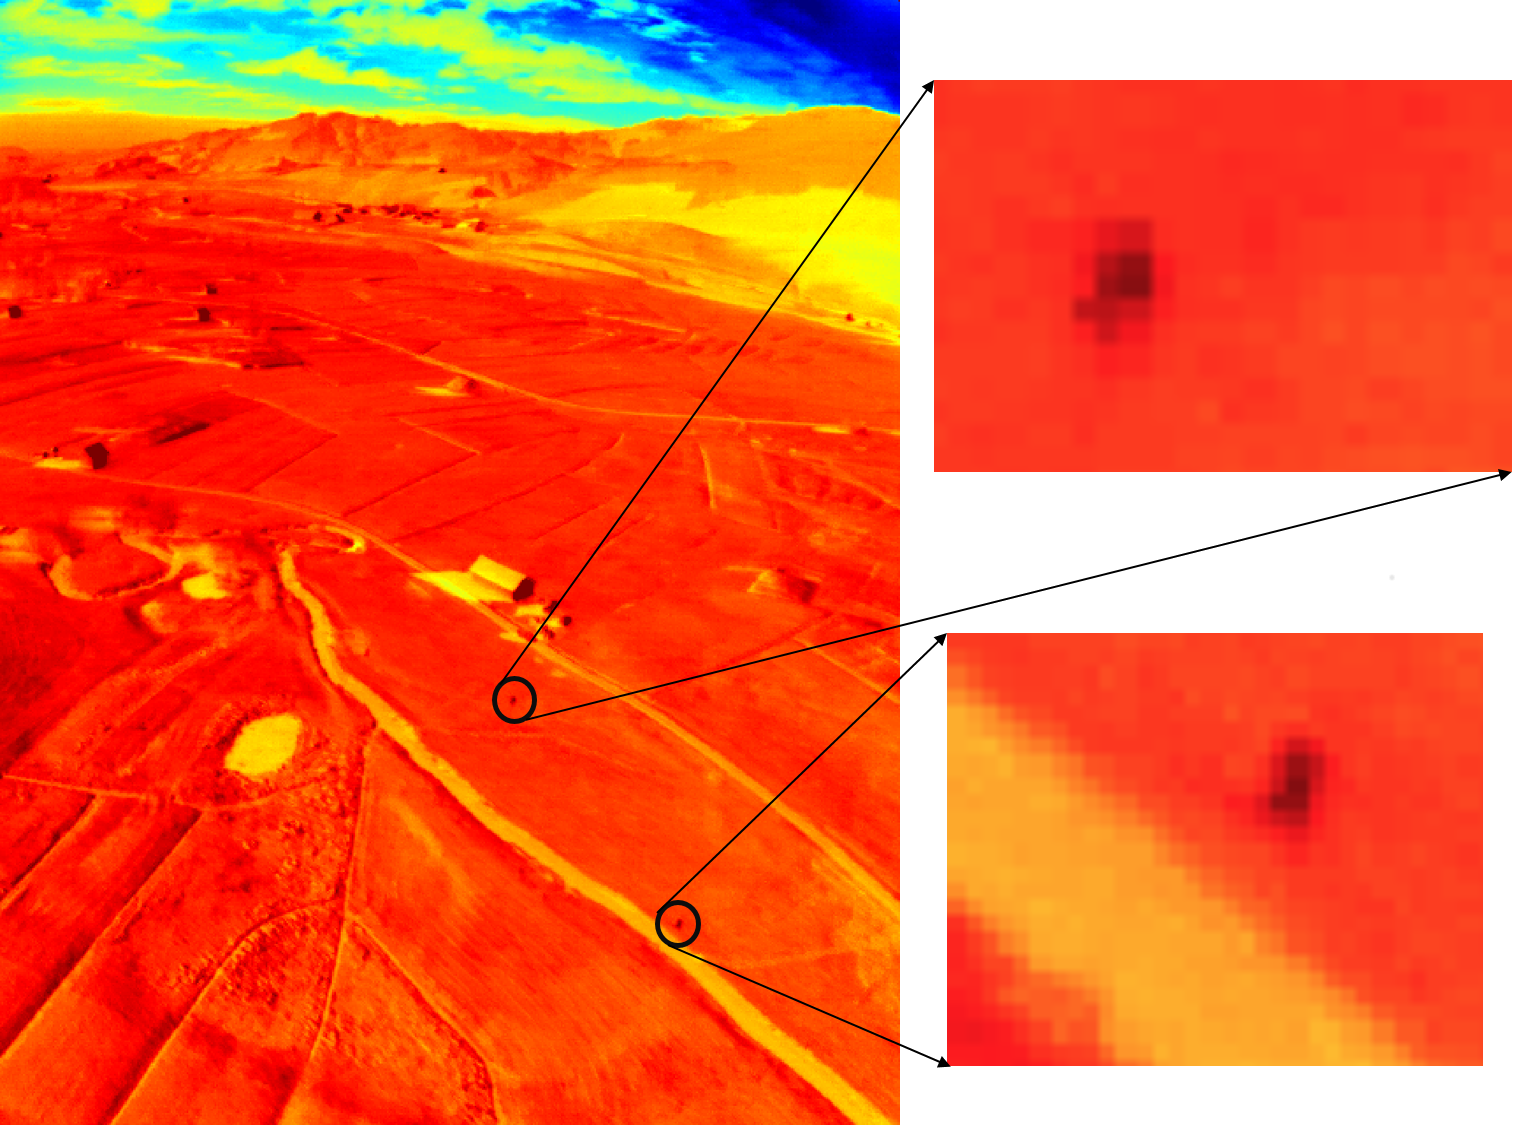
\includegraphics[scale=0.3]{img/sample_thermal.png}}
\caption{A sample image recorded from the FLIR thermal camera at an approximate altitude of 70 meters. Two humans are pointed out.}
\label{fig:thermal_sample}
\end{figure}

We employ a very simple sliding window based approach to estimate adaptive thresholds. The image is divided into various overlapping blocks and the adaptive thresholds $t_{low}^b, t_{high}^b$ for each block $b$ is evaluated as the higher and lower quantiles of the Gaussian models fitted to the pixel intensities of the block. Now, the threshold values at each pixel location $(i, j)$ are chosen as weighted average of all the block thresholds $t_{low}^b, t_{high}^b$ if the pixel belongs to block $b$. The weights are chosen inversely proportional to the pixel's distance from the block's center. A segmentation map (segmap) is generated by thresholding the infrared image at each pixel location.

Fig.~\ref{fig:bg_sub} shows two sample images collected at different altitudes, temperature and times of the day and the corresponding segmaps. A blob detection algorithm \cite{cvblob} is used to find blobs of desired size, thus providing ROIs to search for humans. For the UAV scenario, we further narrow down the search space by considering only the blobs whose area lies in certain range that is calculated at every time-step based on the camera specifications, mounting, UAV's IMU pose and GPS position. This approach is computationally much cheaper and is not affected by the fast moving camera. It provides much faster and better results at real-time than many conventional approaches.


\begin{figure}
  \centering
  \begin{tabular}{ccc}
    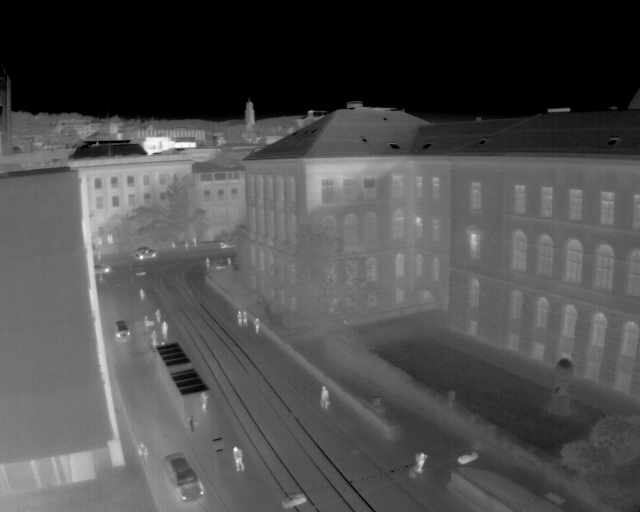
\includegraphics[width=4cm]{img/bg_sub/CLA_Infrared_Image_screenshot_03-08-2015.png} &
    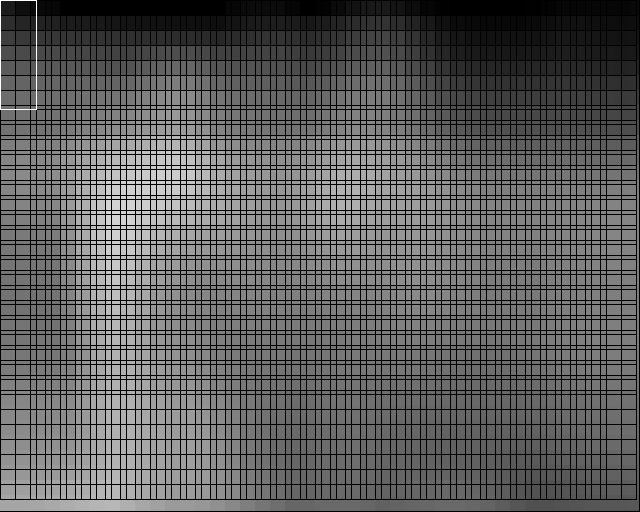
\includegraphics[width=4cm]{img/bg_sub/CLA_Threshold_values(high)_screenshot_03-08-2015.png} &
    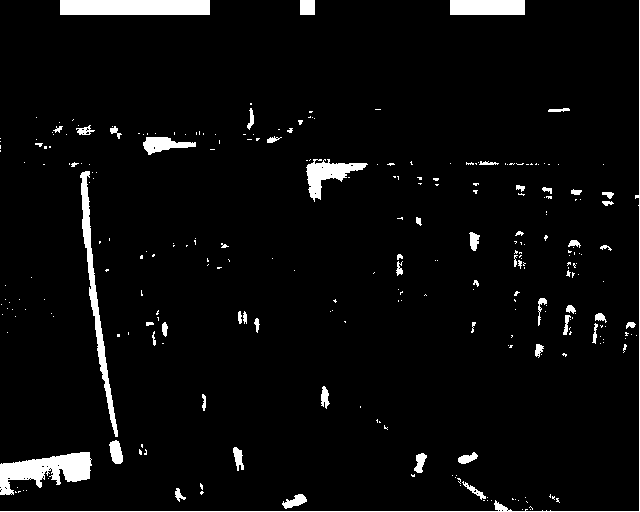
\includegraphics[width=4cm]{img/bg_sub/CLA_Segmentation_Map_screenshot_03-08-2015.png} \\
    \small (1.a) IR image & 
    \small (1.b) 8-bit threshold image &
    \small (1.c) Segmentation map
  \end{tabular}

  \vspace{\floatsep}

  \begin{tabular}{ccc}
    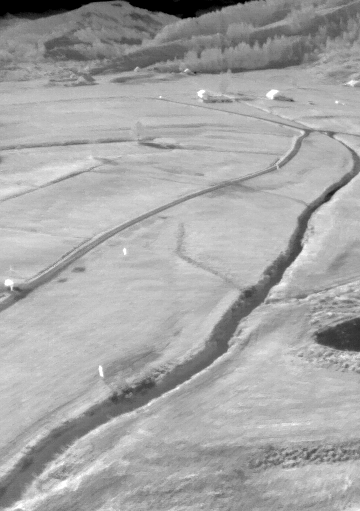
\includegraphics[height=4cm]{img/bg_sub/Roth_Infrared_Image_screenshot.png} &
    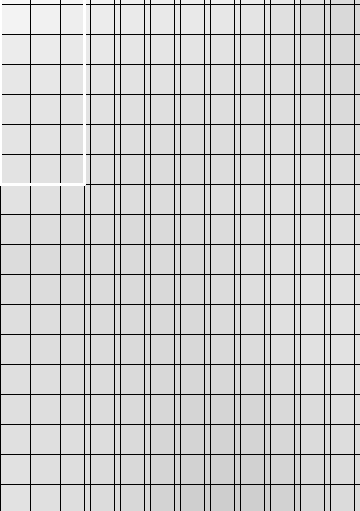
\includegraphics[height=4cm]{img/bg_sub/Roth_Threshold_values(high)_screenshot.png} &
    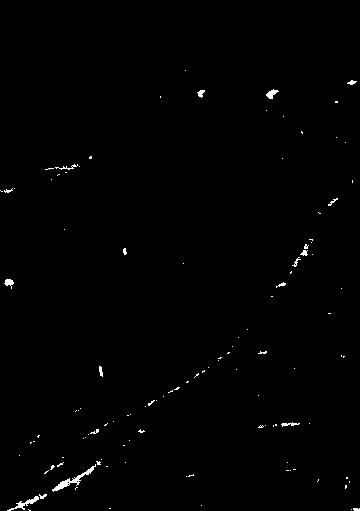
\includegraphics[height=4cm]{img/bg_sub/Roth_Segmentation_Map_screenshot.png} \\
    \small (2.a) IR image & 
    \small (2.b) 8-bit threshold image &
    \small (2.c) Segmentation map
  \end{tabular}

  \caption{Sequence 1 is captured in the night time at an altitude of 20 meters above the ground with some crowd. Sequence 2 was captured from a UAV on a cold winter morning at an altitude of 60 meters above the ground. (a) shows the infrared image, (b) is the 8-bit image of pixel-wise threshold $t_{high}(i, j)$  (grid of blocks is overlaid and a sample block is marked in white on the top-left) and (c) is the resulting segmentation map depicting foreground pixels.}\label{fig:bg_sub}
\end{figure}


\subsection{Human Classifiers}

The ROIs obtained from Background Subtraction are exhaustively searched for presence of a human. For this, we use a HOG feature based learning classifier (which was found to be optimal \cite{portmann2014people}) to classify the extracted patch into human or non-human category. The training data is obtained by manually annotating sequences from different datasets using vBBToolbox \cite{PMT}. HOG features are extracted on the image patches at multiple scales to generate a descriptor. A Support Vector Machine (SVM) classifier is trained using these image patch descriptors. Type of SVM optimization problem, kernel type and other parameters are optimized using K-fold cross validation. Fig.~\ref{fig:k-fold} shows performance of few chosen configurations.

Fig.~\ref{fig:k-fold} shows Precision-Recall curves for the performance of classifier on a validation dataset. The above method is then repeated to train a classifier for grayscale image patches. C\_SVC \cite{svm} optimization problem with Linear kernel type and Radial Basis Function (RBF) kernel type are found to be two top performing configurations for infrared classifier. C\_SVC optimization problem with Linear kernel is found to be optimal configuration for grayscale classifier.

\begin{figure}
  \centering
  \begin{tabular}{m{5cm}m{5cm}m{5cm}}
  \hspace{-1.5cm}
    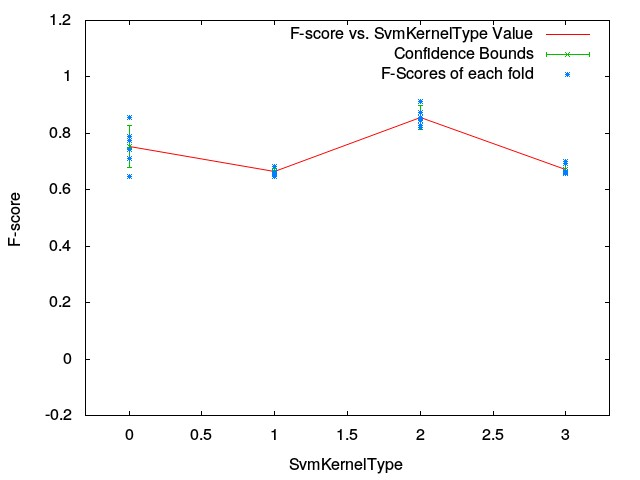
\includegraphics[width=5cm]{img/classifier/SvmKernelTypevalue_vs_score_C_SVC.jpg} &
    \hspace{-1.5cm}
    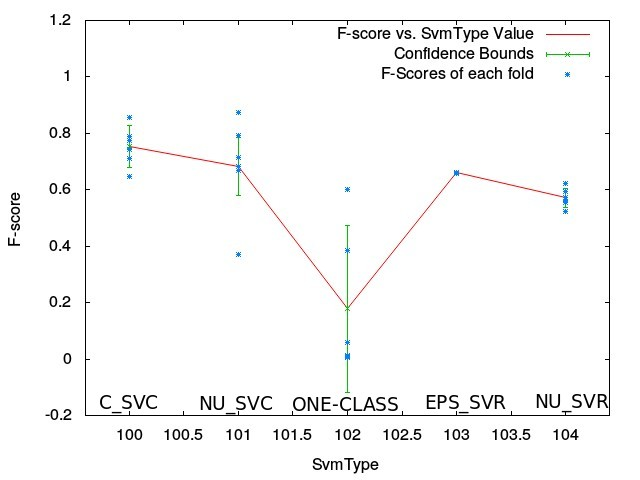
\includegraphics[width=5cm]{img/classifier/SvmTypevalue_vs_score_LINEAR.jpg} &
    \hspace{-1.5cm}
    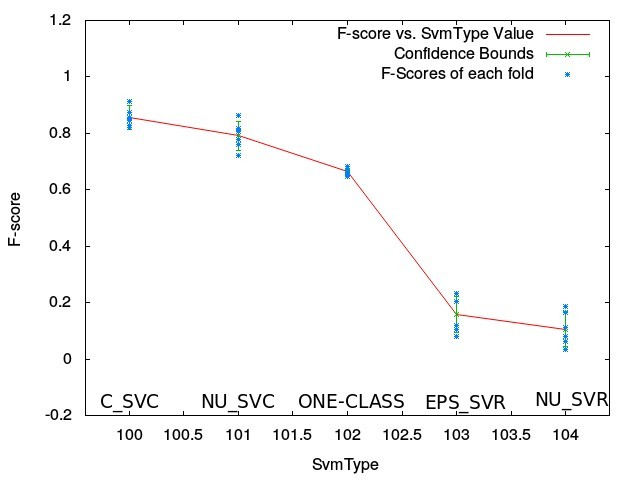
\includegraphics[width=5cm]{img/classifier/SvmTypevalue_vs_score_RBF.jpg} \\
    \hspace{-1.5cm}
    \tiny (a) Choosing kernel type for C\_SVC problem & 
    \hspace{-1.5cm}
    \tiny (b) Choosing optimization for Linear kernel &
    \hspace{-1.5cm}
    \tiny (c) Choosing optimization for RBF kernel
  \end{tabular}
  
  \caption{Performance of infrared SVM classifier with different configurations of optimization problem and kernel type. It's found to be optimal to choose (a) RBF kernel type for C\_SVC problem, (b) C\_SVC problem for Linear kernel type and (c) C\_SVC problem for RBF kernel type.}\label{fig:k-fold}
\end{figure}


\subsection{Infrared-Grayscale Image Fusion} 

Objects in infrared image rarely have discerning features since the temperature tends to be uniform across the objects. So, a classifier would be not so reliable in classifying such patches since it only has the shape information of the object in a very small patch. Since in all our flights using the UAV we collected both infrared and grayscale images, a fusion technique is proposed to get a one to one relationship between pixel locations of infrared and grayscale images. This will help us in extracting both infrared and grayscale image patches corresponding to the ROIs obtained from Background Subtraction which can help the classifier in producing more reliable results.

We use Kalibr \cite{furgale2013unified} to calibrate the infrared and grayscale camera intrinsics and extrinsics for the sensorpod mounting. We use radial-tangential model to estimate camera distortion parameters. An april tag pattern is used to estimate grayscale camera intrinsics. A thick matte paper with checkerboard pattern under illumination of a bright light is used to calibrate infrared camera intrinsics. Now the infrared and grayscale camera setup can be treated as a Stereo pair and standard image rectification techniques \cite{planar_rect} can be used to evaluate the necessary projection matrices. At this point, all the epipolar lines are parallel to image edge (horizontal if horizontal rectification was employed, vertical otherwise). For our particular setup, vertical stereo was chosen since the camera centers were aligned vertically on the UAV. Now that the disparities of the image are in one axis, it's fast and easy to find pixel correspondences. After a manual displacement that is set for all the columns, individual column displacements are evaluated using correspondences between fast features calculated for both the images. A pseudo source code of the image fusion algorithm is listed in List.~\ref{pseudo}.

Once a one-to-one correspondence is obtained between grayscale and infrared images, the patches corresponding to ROIs are passed on to individual human classifiers and pair of patches resulting in high cumulative classifier score are retained for probable presence of a human.


Fig.~\ref{fig:fusion} shows results from the fusion technique. In Sequence-1 infrared and grayscale cameras were both facing in the direction of flight and are in $25^{\circ}$ nadir configuration with a translation of 3.5cm between the camera centers. In Sequence-2, infrared camera was in $25^{\circ}$ nadir configuration while grayscale camera was in $50^{\circ}$ nadir configuration with a translation of 3.5cm between the camera centers. The results show reasonable overlap accuracy. Since we only require a bounding box containing the same object in both infrared and grayscale image, to get corresponding image patches from both images, this level of accuracy suffices.

\begin{figure}
  \centering
  \begin{tabular}{cccc}
    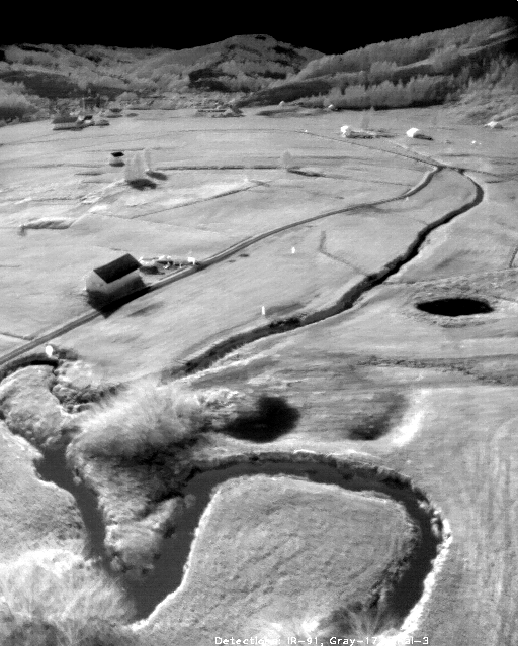
\includegraphics[width=3cm]{img/fusion/Roth/Infrared_Image_screenshot.png} &
    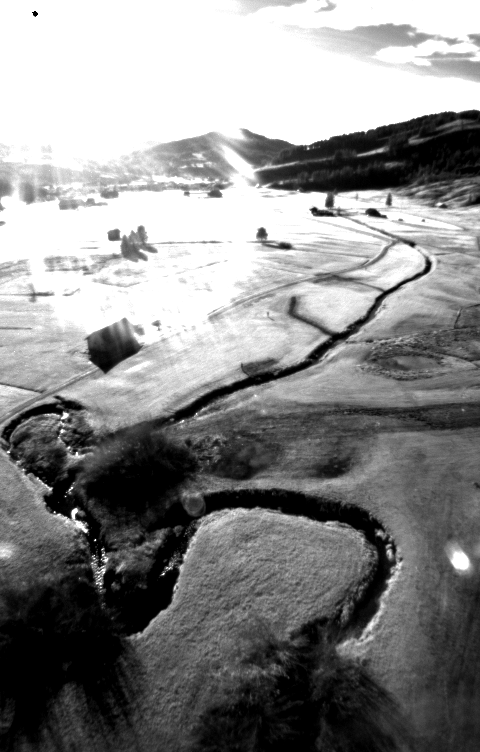
\includegraphics[width=3cm]{img/fusion/Roth/Grayscale_Image_screenshot.png} &
    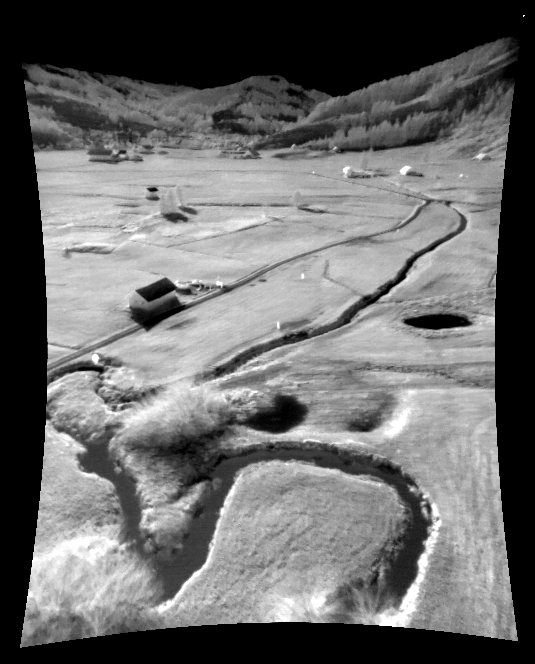
\includegraphics[width=3cm]{img/fusion/Roth/Warped_Infrared_Image_screenshot.png} &
    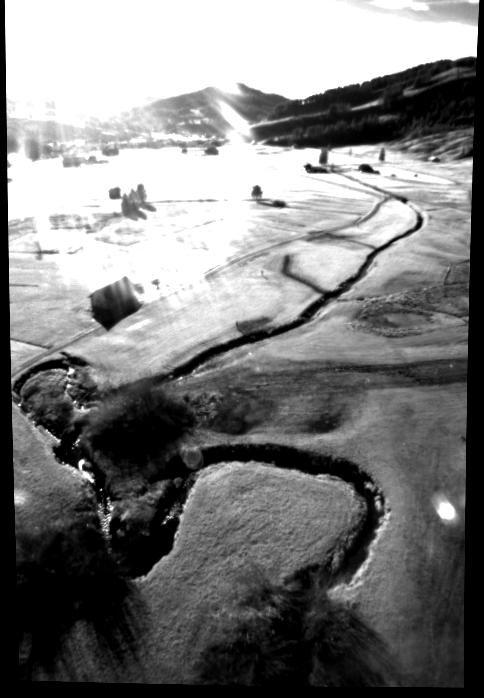
\includegraphics[width=3cm]{img/fusion/Roth/Warped_Grayscale_Image_screenshot.png} \\
    \small (1.a) IR image & 
    \small (1.b) Grayscale Image &
    \small (1.c) Rectified IR &
    \small (1.d) Rectified Grayscale
  \end{tabular}

  \vspace{\floatsep}
  
  \begin{tabular}{cccc}
    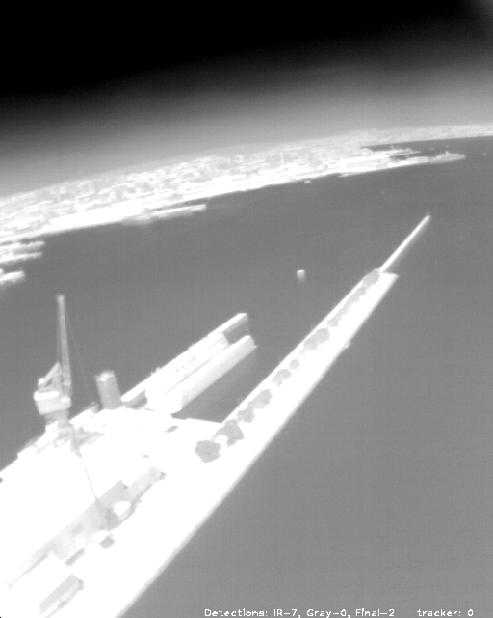
\includegraphics[width=3cm]{img/fusion/Sea/3/Infrared_Image_screenshot.png} &
    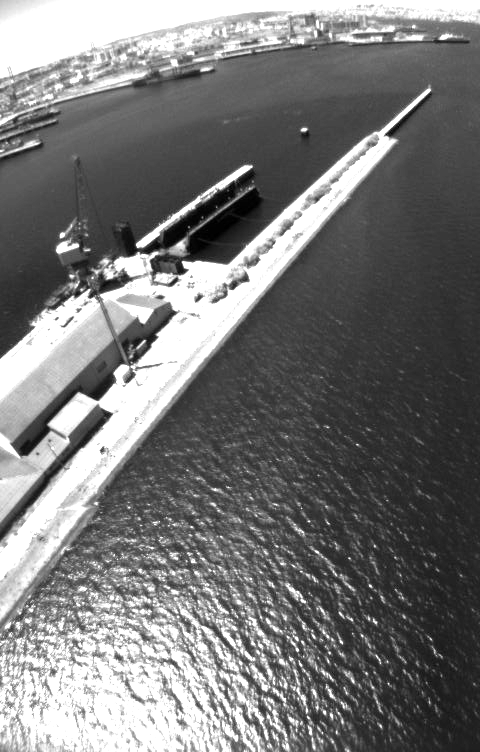
\includegraphics[width=3cm]{img/fusion/Sea/3/Grayscale_Image_screenshot.png} &
    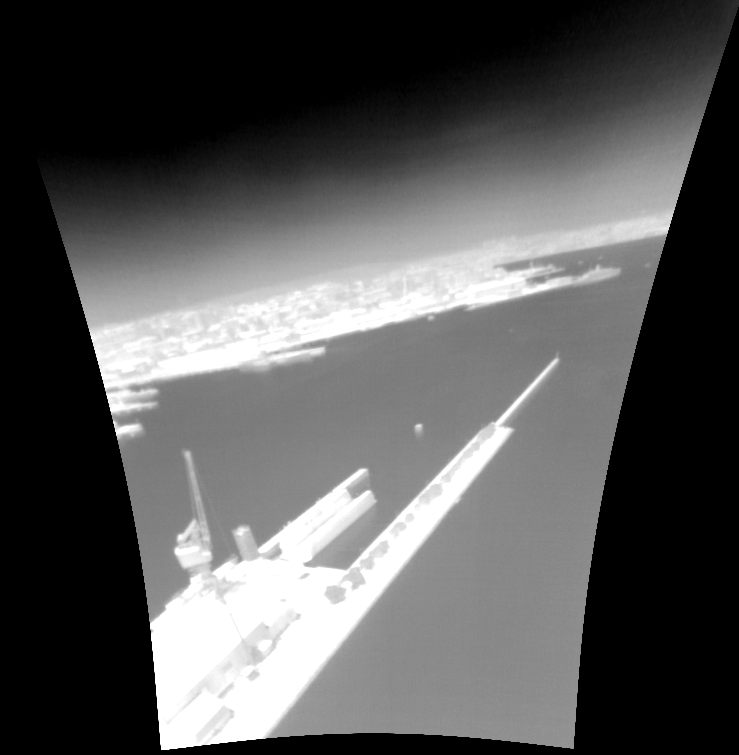
\includegraphics[width=3cm]{img/fusion/Sea/3/Warped_Infrared_Image_screenshot.png} &
    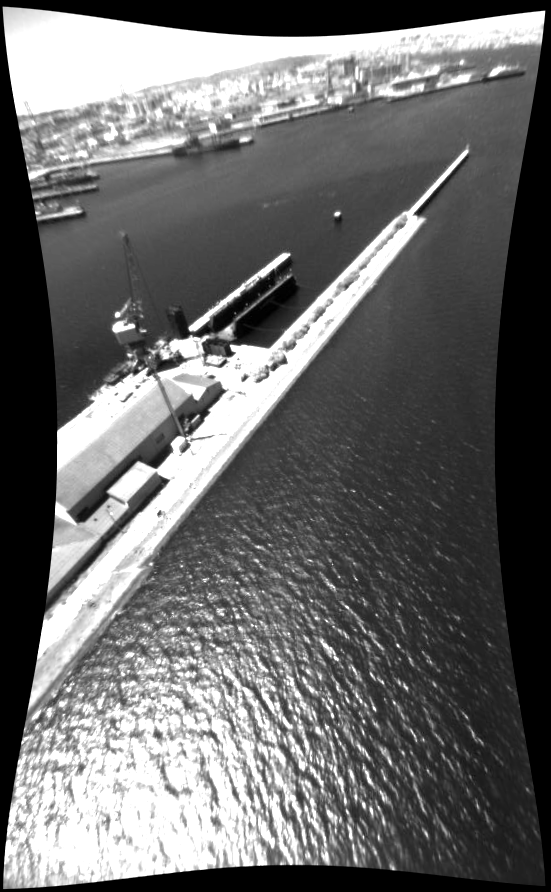
\includegraphics[width=3cm]{img/fusion/Sea/3/Warped_Grayscale_Image_screenshot.png} \\
    \small (2.a) IR image & 
    \small (2.b) Grayscale Image &
    \small (2.c) Rectified IR &
    \small (2.d) Rectified Grayscale
  \end{tabular}
  
  \vspace{\floatsep}
  
  \begin{tabular}{cc}
  	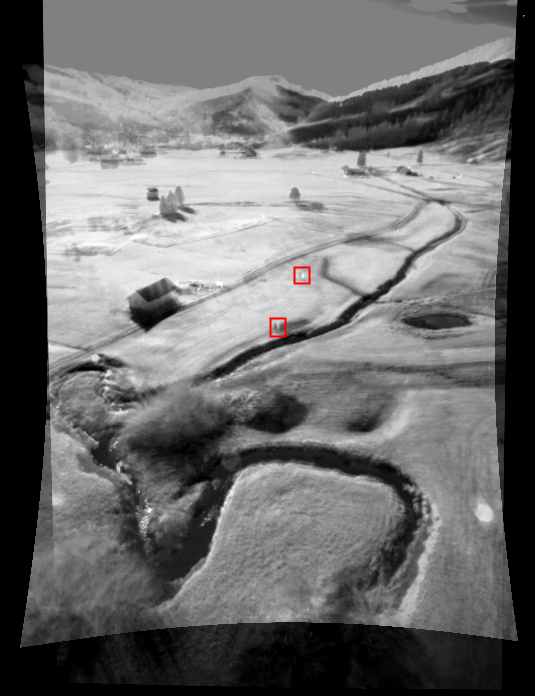
\includegraphics[width=6cm]{img/fusion/Roth/Grayscale_and_Infrared_overlaid_Image_screenshot.png} &
  	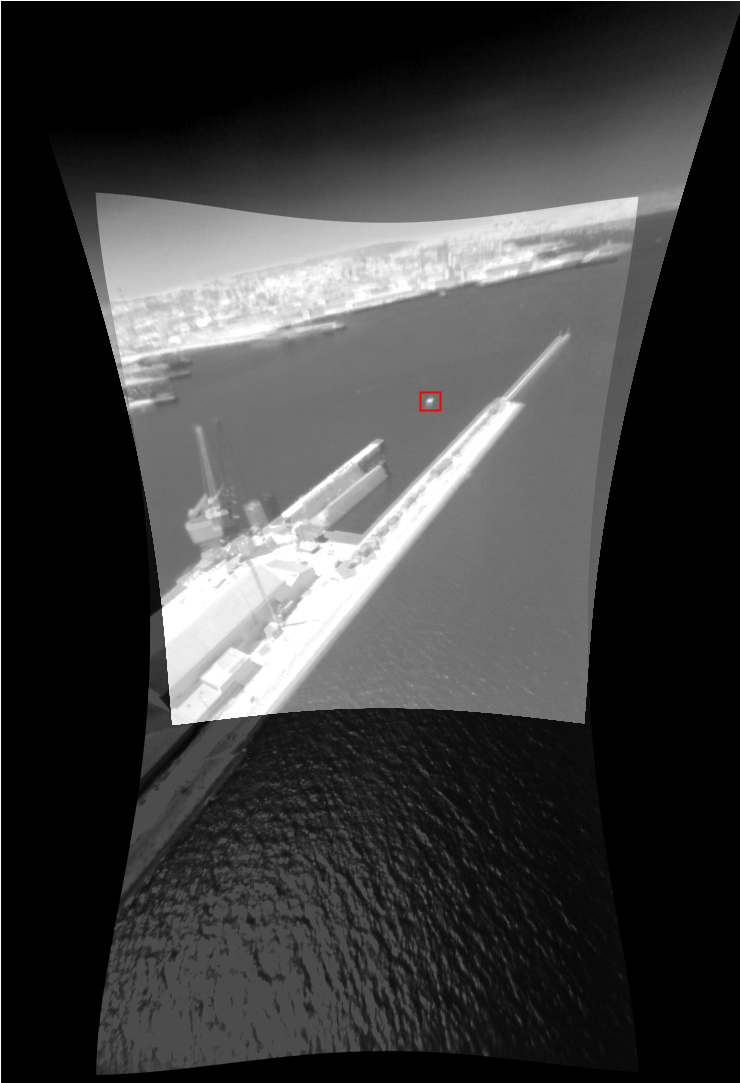
\includegraphics[width=6cm]{img/fusion/Sea/3/Grayscale_and_Infrared_overlaid_Image_screenshot.png} \\
  	\small (1.e) Fused IR and Grayscale Images &
  	\small (2.e) Fused IR and Grayscale Images
  \end{tabular}

  \caption{The top 2 rows show 2 sequences of original images obtained from infrared (a) and grayscale cameras (b) and the resulting images post rectification (c, d). Last row shows fusion of both images (e) to visualize the quality of overlap. Red boxes in Sequence-1 highlights 2 humans and a boat in Sequence-2. As can be seen, the correspondence between infrared and grayscale images is reasonably good.}\label{fig:fusion}
\end{figure}

Fig.~\ref{fig:fusion-pr} shows improvement to the Precision-Recall (PR) curves after image Fusion on a dataset collected from a UAV cruising at 60 meters above the ground. Close to 140\% improvement (10\% vs. 24\%) in the area under curve can be seen. Since, we have various methods to eliminate false positives, as mentioned in next section, we operate our classifier on the higher recall point. Also the fact that very few of the false positives are of a same object recurring across several frames plays a vital role in suppressing them.

\begin{figure}
  \centering
  	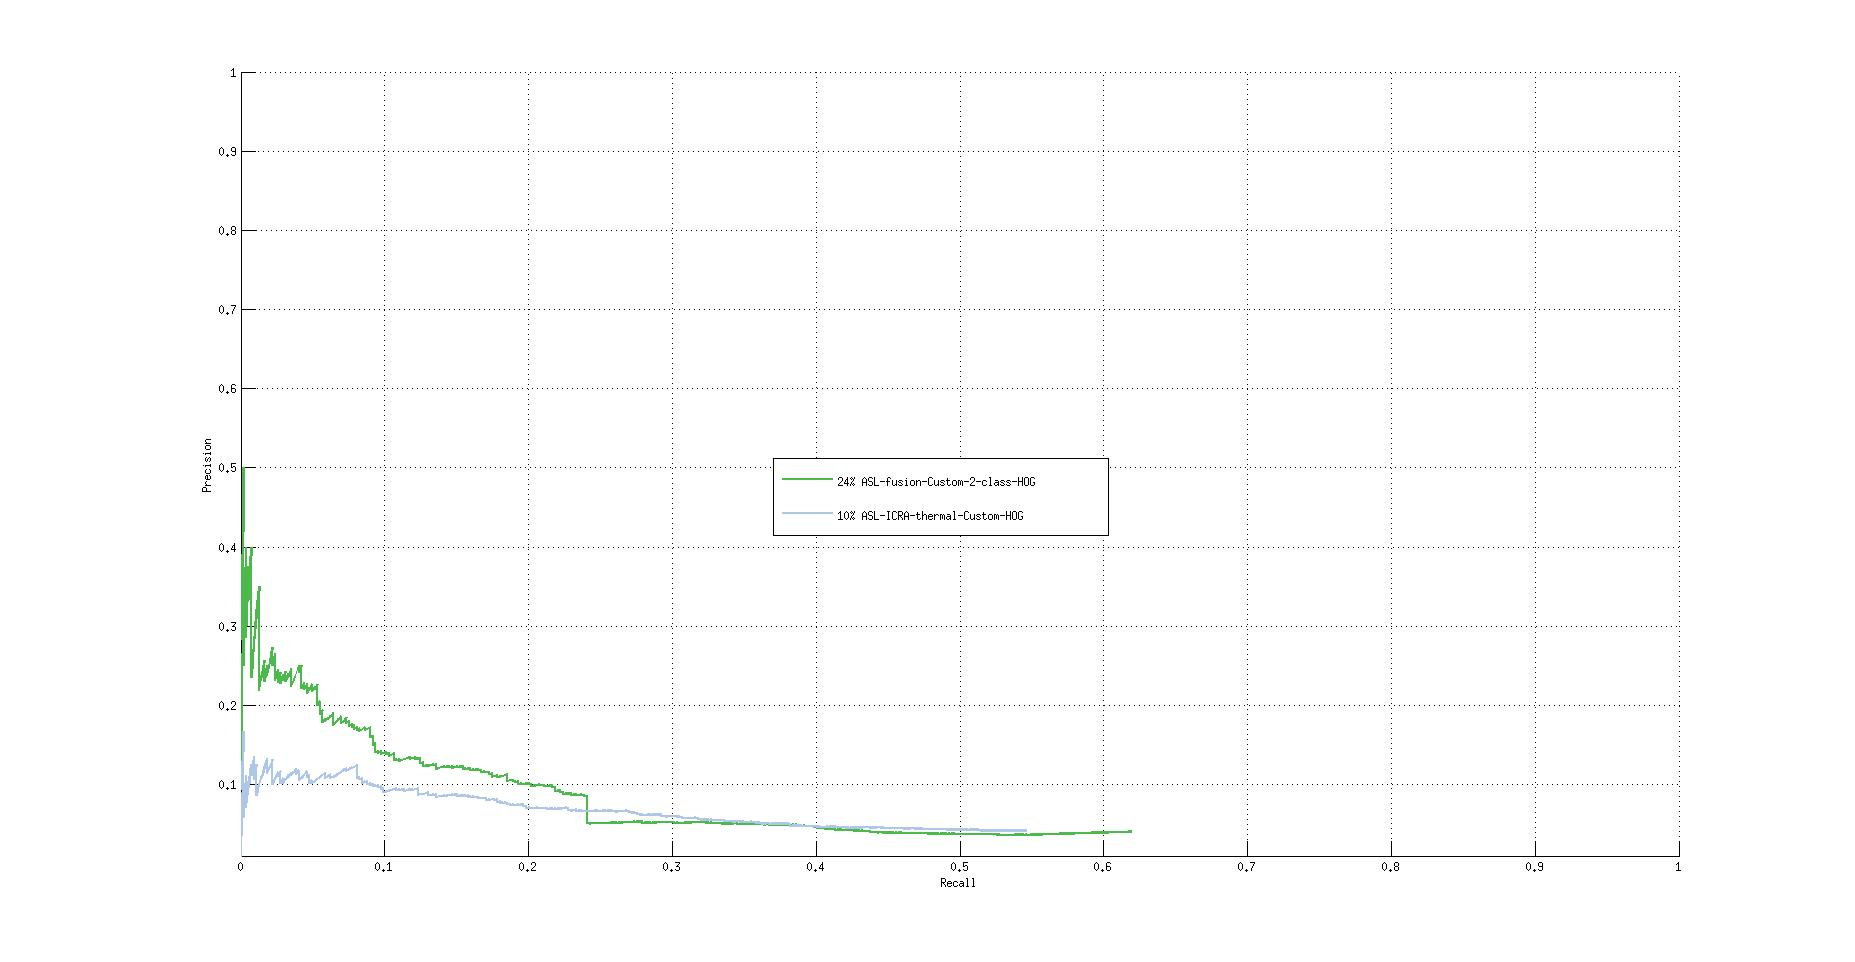
\includegraphics[width=8cm]{img/fusion/Roth/PR-roth-all-detections.jpg} 

  \caption{Precision-Recall curves of the pipeline on a high-altitude (60 meters) data collected from a UAV, before and after image fusion.}\label{fig:fusion-pr}
\end{figure}

\begin{lstlisting}[caption=Pseudo source code for Image fusion, label=pseudo, frame=single]

void (*@\textbf{\sffamily{main}}@*) (int num_arguments, char** arguments) {
  struct Intrinsics {  // Camera Intrinsics.
    cv::Mat_<double> infrared;
    cv::Mat_<double> infrared_distortion;
    cv::Mat_<double> grayscale;
    cv::Mat_<double> grayscale_distortion;
  } intrinsics;
  struct Extrinsics {  // Camera Extrinsics.
    cv::Mat_<double> grayscale_to_infrared;
  } extrinsics;
  struct Rectified {  // Rectified image data.
    // Transformation matrices for rectification.
    cv::Mat_<double> grayscale_transform;
    cv::Mat_<double> infrared_transform;
    // New optimal camera matrices.
    cv::Mat_<double> new_grayscale_intrinsics; 
    cv::Mat_<double> new_infrared_intrinsics;
    cv::Mat_<double> intrinsics;
  } rectified;
  struct Mappings {  // Transformation mappings.
    // Transformation maps for rectified images. transformed_image(x, y) = image(map(x, y)).
    cv::Mat infrared;
    cv::Mat grayscale;
    bool evaluated = false;
    cv::Mat offsets;  // Offsets to align rectified images.
  } mappings;

  (*@\textbf{\sffamily{loadCalibration}}@*)(intrinsics,extrinsics);  // Load camera intrinsics.
  // Generate new optimal camera intrinsics that will ensure maximum possible number of pixels of both images are retained after un-distortion, in destination image size same as the original image.
  rectified.new_infrared_intrinsics = cv::(*@\textbf{\sffamily{getOptimalNewCameraMatrix}}@*)(
    intrinsics.infrared,intrinsics.infrared_distortion,infrared_image_size);
  rectified.new_grayscale_intrinsics = cv::(*@\textbf{\sffamily{getOptimalNewCameraMatrix}}@*)(
    intrinsics.grayscale,intrinsics.grayscale_distortion,grayscale_image_size);
  // Obtain single optimal camera matrix that ensures all the pixels from both the images are retained post un-distortion.
  rectified.intrinsics = (*@\textbf{\sffamily{getOptimalNewCameraMatrix}}@*)(
    rectified.new_infrared_intrinsics,rectified.new_grayscale_intrinsics);
  // Compute rectification transforms for each camera in the calibrated stereo pair using OpenCV Stereo Rectification.
  cv::(*@\textbf{\sffamily{stereoRectify}}@*)(
    intrinsics.infrared,intrinsics.infrared_distortion,
    intrinsics.grayscale,intrinsics.grayscale_distortion,
    extrinsics.grayscale_to_infrared,rectified.infrared_transform,
    rectified.grayscale_transform);

  while (incoming ROS messages) {
    // Read ROS infrared image message.
    if (message_view.getTopic() == infrared_topic) {
      cv::Mat infrared = (*@\textbf{\sffamily{getImage}}@*)(message_view); // Read the image.
    }
    // Read ROS grayscale image message.
    if (message_view.getTopic() == grayscale_topic) {
      cv::Mat grayscale = (*@\textbf{\sffamily{getImage}}@*)(message_view); // Read the image.
      // Evaluate transformation maps using computed destination camera matrix and the stereo rectification transforms.
      if ( !mappings.evaluated ) {
        cv::(*@\textbf{\sffamily{initUndistortRectifyMap}}@*)(
          intrinsics.infrared,intrinsics.infrared_distortion, 
          rectified.infrared_transform,rectified.infrared_intrinsics, 
          rectified.destination_size,mappings.infrared);
        cv::(*@\textbf{\sffamily{initUndistortRectifyMap}}@*)(
          intrinsics.grayscale,intrinsics.grayscale_distortion,
          rectified.grayscale_transform,rectified.infrared_intrinsics,
          rectified.destination_size,mappings.grayscale);
        mappings.evaluated = true;
      }
      // Apply offsets to transformation maps using robust feature matching.
      cv::(*@\textbf{\sffamily{goodFeaturesToTrack}}@*)(infrared,infrared_features);
      cv::(*@\textbf{\sffamily{goodFeaturesToTrack}}@*)(grayscale,grayscale_features);
      (*@\textbf{\sffamily{findOffsets}}@*)(infrared_features,grayscale_features,mappings.offsets);
      (*@\textbf{\sffamily{applyOffsets}}@*)(mappings.offsets,mappings.infrared,mappings.grayscale);    
      // Rectify the images.
      cv::(*@\textbf{\sffamily{remap}}@*)(infrared,rectified_infrared,mappings.infrared);
      cv::(*@\textbf{\sffamily{remap}}@*)(grayscale,rectified_grayscale,mappings.grayscale);
    }
    // Remap the ROIs into rectified image and extract overlapping patches in both the images corresponding to the new ROIs.
    new_ROI = (*@\textbf{\sffamily{remapRect}}@*)(ROI,mappings.infrared);
    infrared_image_patch = rectified_infrared(new_ROI);
    grayscale_image_patch = rectified_grayscale(new_ROI);
  }
}
\end{lstlisting}


\section{Experimental Results}

Inspired by real-world search and rescue initiatives, we designed a representative field trial utilising our full aerial deployment and victim detection pipeline. The experiment involves the placement of multiple ``victims" throughout a field over which our rapidly deployable, hand launched, fixed-wing test platform, equipped with multi-camera carrying sensorpod, must survey in a timely manner and record GPS coordinates of victims seen during the flight. In the following sections, we present the setup, enabling tools, and results.

\subsection{Platform Description}

All the experiments are performed on a light-weight low-altitude hand-launchable fixed-wing UAV that is mounted with a sensorpod. [wing span, weight, cruise speed]. The UAV also consists of various telemetry, inertial modules and employs an open-source Pixhawk PX4 Autopilot \cite{meier2015px4} system. The sensorpod is equipped with rigidly connected infrared (FLIR Tau 2) and grayscale (Aptina MT9V034) cameras with oblique field-of-view, IMU (Analaog Devices ADIS16448), Skybotix VISensor \cite{Skybotix} and a computer with an Intel Atom processor.

\subsection{Full coverage aerial inspection}

To ensure victims are seen by the cameras' fields of view at some point during the flight, we employ a fast inspection planning algorithm which guarantees full coverage of a mesh-model world (obtained from GIS data) to ensure all ground is scanned for victims. The algorithm, details in \cite{7140101}, employs an iterative viewpoint re-sampling technique, using randomized sampling, to provide viewpoint configurations that maintain full coverage while simultaneously searching for the best route that visits them all, using the Lin-Kernighan heuristic \cite{lin1973effective}. Nonholonomic vehicle constraints and obstacle avoidance are further considered in the path search using a boundary value solver in combination with the Rapid Random Tree (RRT*) motion planner \cite{RRTS1a}. The path generated (see Fig.~\ref{fig:victim_gps}(a)) for this experiment ensured coverage of $~$52,800 sq. meters with a flight time of just under two minutes.

\subsection{Estimating victim GPS}

For estimating the GPS positions of detections, we assume the ground as a plane. Using camera intrinsics and detection's pixel location, we find the directional vector in which the object might be lying. The point where this vector hits the ground plane can be found using GPS, IMU and camera-IMU extrinsics data which finally gives victim's GPS location.

Fig.~\ref{fig:victim_gps}(b) shows the detected victim GPS positions, actual groundtruth victim location and the path followed by the UAV. The rest of the detections include unregistered humans in the explored area and some false positives. By enforcing a criterion - similar to \cite{rudol2008human} - that requires a particular GPS position to be detected consistently within the duration of the time that particular spot is observed, most of the false positives are eliminated and the set of true detections are grouped together and registered as victim locations. False positives are further eliminated by boosting the confidence of detections that are closer to the GPS location of the point where principal axis of camera hits the ground plane. The registered victims are marked in circles. As can be seen in the figure, we have all three successful detections and another detection whose status is not known. Fig.~\ref{fig:victim_gps}(c) is a plot of GPS position estimate errors for all the three registered victims. The GPS estimates are converted to Universal Transverse Mercator (UTM) coordinates using World Geodetic System (WGS84) standard \cite{WGS} to represent the error in meters. The errors obtained are a cumulative of errors in groundtruth GPS measuring device, calibration imperfections, GPS to/from UTM conversions, images' resolution, planarity assumptions, and sensor imperfections (GPS, IMU), making it quite uncertain how much of the error can be attributed to the imperfections in our algorithm. Nevertheless, the errors we obtained more than suffice to serve our goal. The only assumption made in our approach is of ground planarity and even this can be easily overcome by using geographical elevation data of the scanned region.


\begin{figure}
  \centering
  \begin{tabular}{cc}
    \hspace{-1cm}
    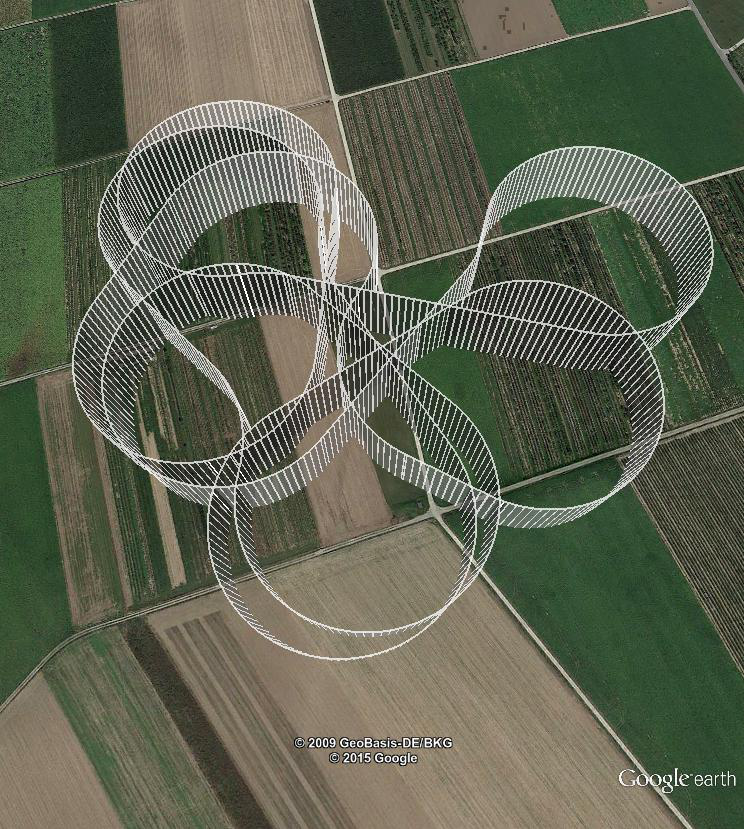
\includegraphics[width=7cm]{img/victim_gps/SIP.png} &
    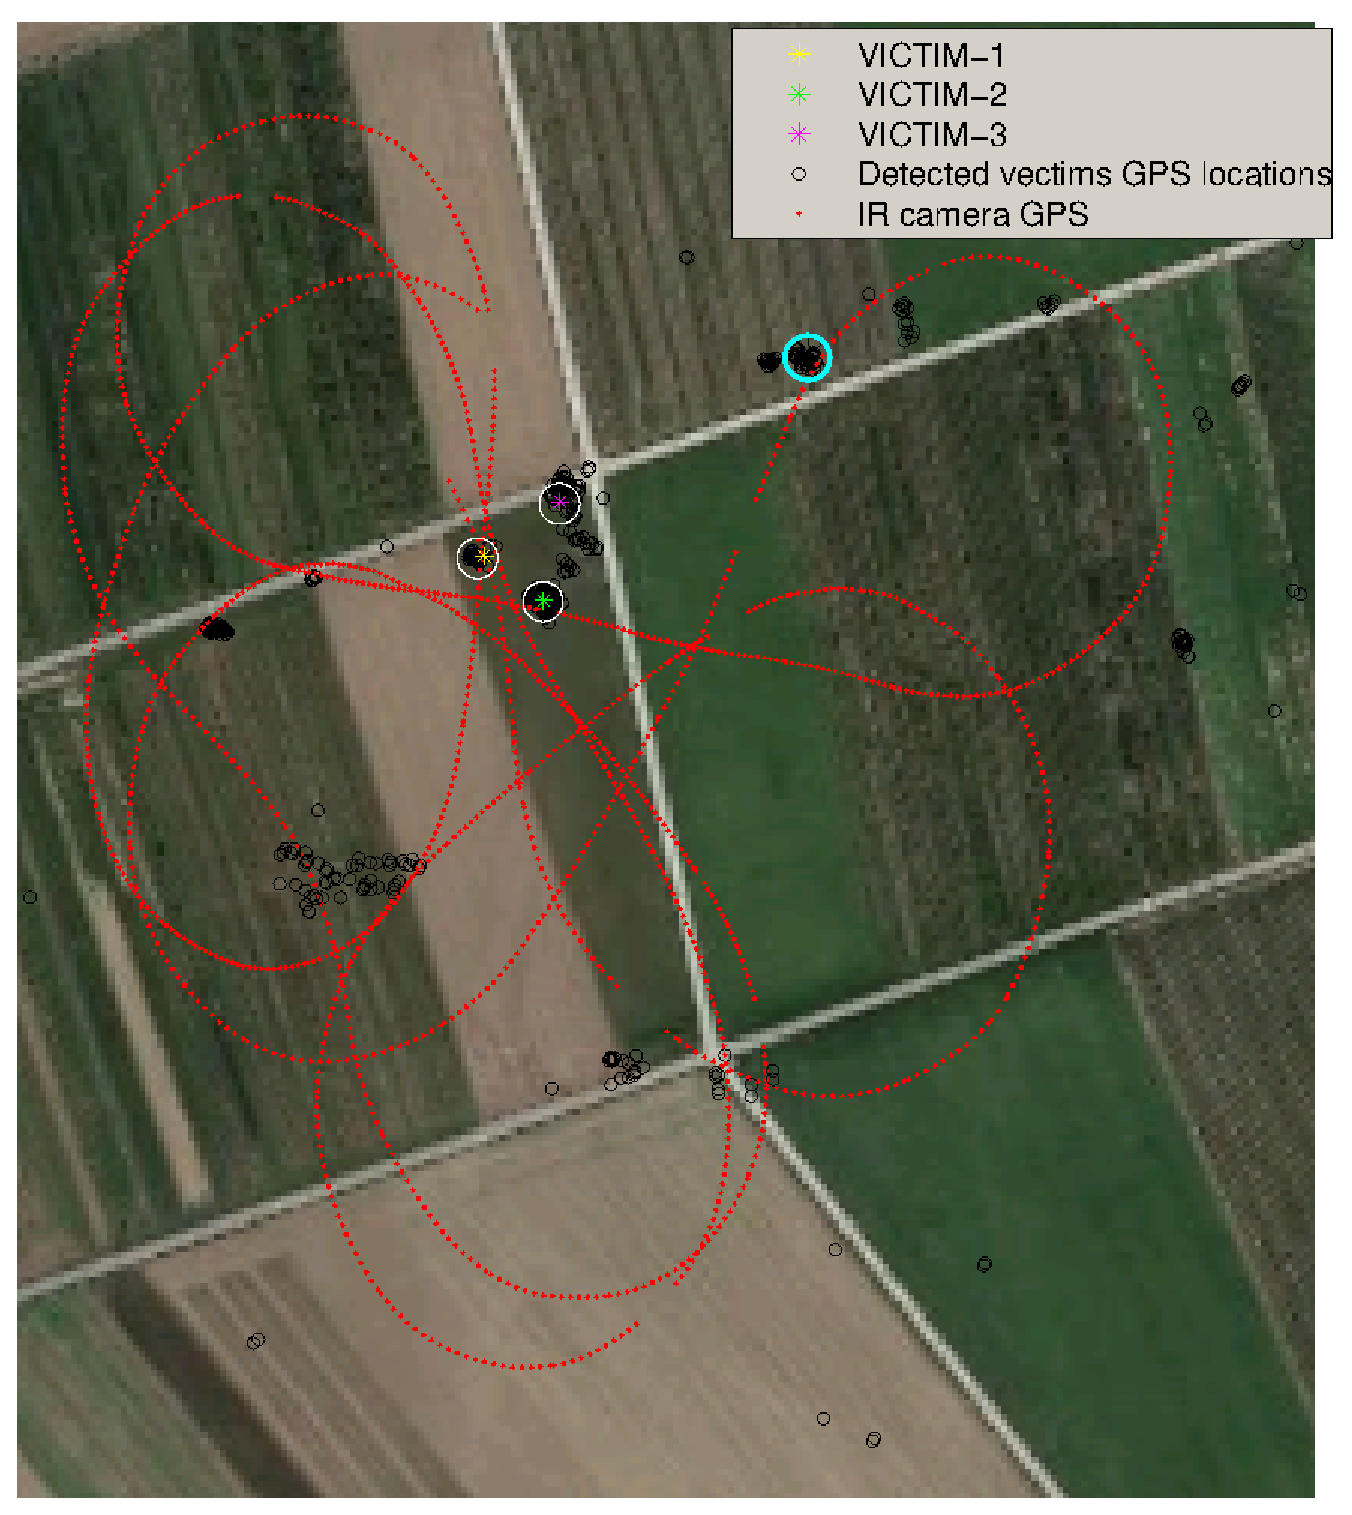
\includegraphics[width=7cm]{img/victim_gps/SIP_detections_map.eps} \\
    \small (a) Inspection path & 
    \small (b) Victim GPS \tiny (Grouped detections in circle after false positive removal)
  \end{tabular}

  \vspace{\floatsep}
  
  \begin{tabular}{c}
    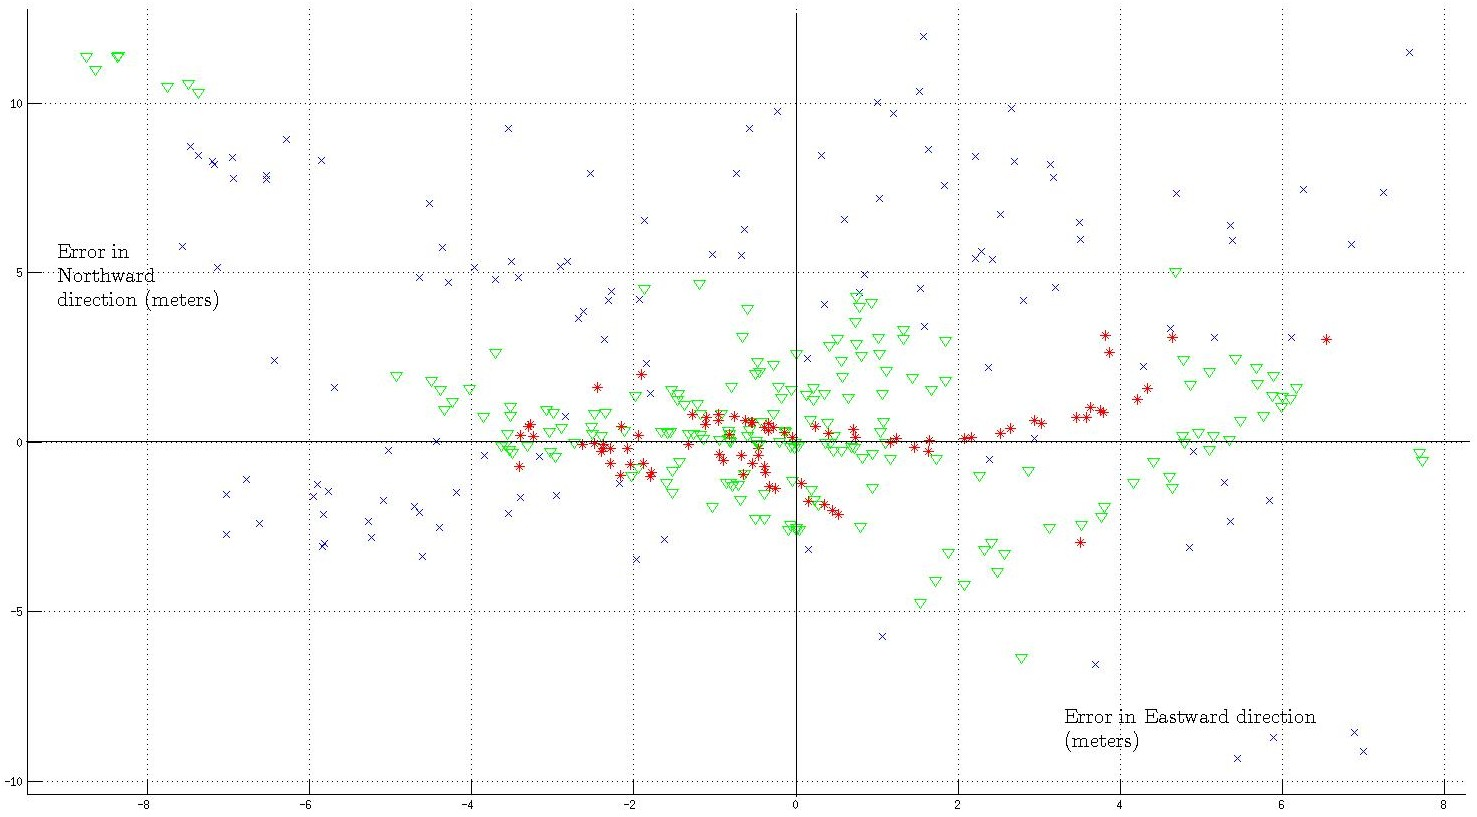
\includegraphics[width=11cm]{img/victim_gps/victim_utm_errors.jpg} \\
    \small (c) Victim UTM position errors
  \end{tabular}

  \caption{Full coverage field test detection results.}\label{fig:victim_gps}
\end{figure}



\section{Conclusions and Future Work}

At present, we have many parameters that need to be set manually. In the future, we plan to have some adaptive estimation of these values. Computing HOG descriptors for each foreground patch is quite time consuming as well. Instead, using a weak classifier with high recall could reduce computation times, as our pipeline has the ability to deal with classifier false positives. We also plan to track the detections in UTM coordinates to have consistent detections of moving targets. Use of elevation data would also be a way to remove the planar ground assumption currently implemented and improve detection location estimations. In all, we have shown, as a proof of concept, that human victim detection from upwards of 50-60 meters via a fast moving fixed-wing aircraft is possible. Further, we have demonstrated the algorithm's real-time capacity for victim detection and localisation in a real-world search scenario.

%-----------------------------------------------------------------
%	Acknowledgements  
%-----------------------------------------------------------------
\section*{Acknowledgements}

This work was supported by the European Commission projects ICARUS (\#285417) and SHERPA (\#600958) under the 7th Framework Programme.

\nocite{bal:cha:gra:pae}
\bibliographystyle{splncs}
\bibliography{isvc_submission}

\end{document}
